% Provenance (never printed): see sources/outline_sources.md (Year 1: fault types and
% Anderson's theory; fold geometry and classification; foliation, schistosity and
% lineation; microstructures). Exercise and problem values in the Book 3 scratch calculator
% calc/ch17.py; the Varden Hills fold and fault from figdata/shared/region.py (read only).
% Fold, anticline, syncline and fold axis are owned by ch. 4; throw and heave by ch. 5;
% trend and plunge by ch. 6; the stresses and the Coulomb criterion by ch. 16. Shear zones
% and deformation mechanisms belong to the Year 3 volume (told here).
\chapter{Falhas, dobras e fábricas}\label{ch:b1:faults-folds-fabrics}

Um corte de estrada mostra uma face de rocha polida como vidro e riscada por sulcos paralelos finos. Do outro lado do vale, um penhasco à beira-mar mostra camadas de arenito e de folhelho dobradas em ziguezagues de lados retos e cantos vivos. Num telhado próximo, ardósias se partem em lâminas de poucos milímetros de espessura, ao longo de planos que cortam as camadas da lama de que foram feitas. Cada um é um registro da deformação da rocha, lido em uma escala diferente: os sulcos dão a \omterm{def:b1:geological-maps:attitude}{direção} em que dois blocos deslizaram um ao longo do outro, numa falha; os ziguezagues medem quanto as camadas foram encurtadas; os planos da ardósia cresceram atravessando a textura da rocha enquanto ela era comprimida. Este capítulo dá a geometria necessária para medir os três registros, e a mecânica do capítulo anterior explica por que as falhas tomam os \omterm{def:b1:geological-maps:attitude}{mergulhos} que tomam.

\begin{recall}
A \omterm{def:b1:geological-maps:attitude}{atitude} de um plano é seu \omterm{def:b1:geological-maps:attitude}{sentido de mergulho} e seu \omterm{def:b1:geological-maps:attitude}{mergulho}, escrita por exemplo como $080/12$; sua \omterm{def:b1:geological-maps:attitude}{direção} segue pela regra da mão direita, o plano mergulhando para a direita de um observador que olha ao longo da \omterm{def:b1:geological-maps:attitude}{direção} (\cref{ch:b1:geological-maps}). Uma \omterm{def:b1:geological-maps:fold}{dobra} é uma curvatura de camadas originalmente planas; um \omterm{def:b1:geological-maps:fold}{anticlinal} é convexo para cima, com as rochas mais antigas no núcleo, e um \omterm{def:b1:geological-maps:fold}{sinclinal} é côncavo para cima; o eixo da \omterm{def:b1:geological-maps:fold}{dobra} é a linha ao longo da qual as camadas mais se curvam (\cref{ch:b1:geological-maps}). O \omterm{def:b1:cross-sections:throw}{rejeito} e o salto de uma falha são as componentes vertical e horizontal de seu deslocamento (\cref{ch:b1:cross-sections}). Uma linha tem um \omterm{def:b1:field-lab-methods-1:trend-plunge}{rumo} de \omterm{def:b1:field-lab-methods-1:trend-plunge}{caimento} e um \omterm{def:b1:field-lab-methods-1:trend-plunge}{caimento}, e o vetor unitário para baixo $(\cos p\sin t, \cos p\cos t, -\sin p)$ (\cref{ch:b1:field-lab-methods-1}). Uma rocha que obedece ao critério de Coulomb rompe-se em planos a $\ang{45} - \phi/2$ de $\sigma_1$, e falhas existentes deslizam segundo a \omterm{prop:b1:stress-strain-rheology:byerlee}{lei de Byerlee} (\cref{ch:b1:stress-strain-rheology}). Um \omterm{def:b1:rock-forming-minerals:mineral}{mineral} está em extinção entre \omterm{def:b1:field-lab-methods-1:microscope}{polarizadores cruzados} quando suas direções de vibração são paralelas às dos polarizadores (\cref{ch:b1:optical-mineralogy}). Falhas foram vistas no Livro 1, 7º ano; \omterm{def:b1:faults-folds-fabrics:fault-types}{falhas inversas}, empurrões e \omterm{def:b1:faults-folds-fabrics:foliation}{xistosidade} no Livro 2, 12º ano. O produto vetorial de dois vetores é perpendicular a ambos (matemática, primeiro ano).
\end{recall}

\section{Falhas: geometria e cinemática}\label{sec:b1:faults-folds-fabrics:faults}

Uma falha é uma superfície ao longo da qual dois blocos de rocha deslizaram um em relação ao outro. Para descrever o movimento precisamos de nomes para os dois blocos e para o deslocamento, e de um modo de medir sua \omterm{def:b1:geological-maps:attitude}{direção} dentro do plano da falha.

\begin{definition}[Bloco superior, bloco inferior, vetor de deslizamento, deslizamento líquido, rake]\label{def:b1:faults-folds-fabrics:fault-elements}
Seja uma falha localmente um plano que não é vertical. O \emph{bloco superior}\index{bloco superior} é o bloco acima dela, o \emph{bloco inferior}\index{bloco inferior} o bloco abaixo. Seja $A$ um ponto do bloco inferior e $A'$ o ponto do bloco superior que estava em contato com ele antes do movimento. O \emph{vetor de deslizamento}\index{vetor de deslizamento} $\overrightarrow{AA'}$ é o deslocamento do bloco superior em relação ao inferior; seu comprimento é o \emph{deslizamento líquido}\index{deslizamento líquido}. O \emph{rake}\index{rake} $r$ (também chamado pitch) do vetor de deslizamento é o ângulo, medido no plano da falha, desde a \omterm{def:b1:geological-maps:attitude}{direção} dada pela regra da mão direita até o vetor de deslizamento, positivo quando o vetor aponta para cima do plano e negativo quando aponta para baixo: $\ang{-180} < r \le \ang{180}$. Esta é a convenção dos sismólogos, usada de novo para terremotos em \cref{ch:b1:earthquake-source}; muitos geólogos de campo registram, em vez disso, um ângulo entre 0 e \ang{180}, medido no sentido horário a partir da \omterm{def:b1:geological-maps:attitude}{direção} vista de cima, e acrescentam o sentido do movimento em palavras.
\end{definition}
% ledger: ar:rake, ws:rake, ws:fault-terms

Os dois nomes vêm da mineração: um mineiro que trabalhava um filão inclinado ficava sobre o \omterm{def:b1:faults-folds-fabrics:fault-elements}{bloco inferior} e tinha o \omterm{def:b1:faults-folds-fabrics:fault-elements}{bloco superior} sobre a cabeça. Um deslocamento visto em um único corte não é, em geral, o deslizamento: uma camada deslocada em um mapa ou em uma seção mostra uma separação, que depende da \omterm{def:b1:geological-maps:attitude}{atitude} da camada. O deslizamento precisa de dois pontos que foram um só, como as duas metades de uma linha cortada pela falha, por exemplo a borda de um dique contra uma camada.

\begin{omfigure}
\begin{tikzpicture}[>={Stealth[length=5pt]}, font=\small]
% (a) the fault plane seen face-on; slip vector of length 3.6 cm at rake -35 deg
% (normal and sinistral): strike-slip component 3.6 cos 35 = 2.949, dip-slip 3.6 sin 35 = 2.065
\pgfmathsetmacro{\Ls}{3.6*cos(35)}\pgfmathsetmacro{\Ld}{3.6*sin(35)}
\begin{scope}
  \fill[omDef!15] (0,0) rectangle (6.2,3.4);
  \draw[omDef, line width=0.7pt] (0,0) rectangle (6.2,3.4);
  \draw[line width=1.2pt] (0,3.4) -- (6.2,3.4);
  \node[anchor=south, font=\scriptsize] at (3.1,3.4) {linha de direção, onde a falha encontra o solo};
  \draw[->, line width=0.6pt] (6.45,3.0) -- (6.45,2.0) node[midway, right, font=\scriptsize, align=left] {para baixo\\ no mergulho};
  \draw[->, line width=0.6pt] (0.3,0.35) -- (1.3,0.35) node[right, font=\scriptsize] {direção};
  \coordinate (A) at (1.2,2.55);
  \coordinate (B) at ($(A)+(\Ls,0)$);
  \coordinate (A2) at ($(A)+(\Ls,-\Ld)$);
  \draw[omProp, dashed, line width=0.7pt] (A) -- (B) node[midway, above, font=\scriptsize] {componente transcorrente};
  \draw[omProp, dashed, line width=0.7pt] (B) -- (A2) node[midway, right, font=\scriptsize, align=left] {componente de\\ mergulho};
  \draw[->, line width=1.3pt, omThm] (A) -- (A2) node[midway, below left, font=\scriptsize, inner sep=1pt] {vetor de deslizamento};
  \draw[black] ($(A)+(0.9,0)$) arc[start angle=0, end angle=-35, radius=0.9];
  \node[font=\scriptsize] at ($(A)+(-17.5:1.15)$) {$r$};
  \fill (A) circle[radius=1.4pt] node[above left, inner sep=1.5pt] {$A$};
  \fill (A2) circle[radius=1.4pt] node[below right, inner sep=1.5pt] {$A'$};
  \node[font=\small\bfseries] at (3.1,-0.55) {(a) no plano da falha};
\end{scope}
% (b) the vertical section through the dip line: dip 50 deg; dip-slip 2.065 -> throw 1.582, heave 1.327
\begin{scope}[xshift=9.4cm, yshift=0.2cm]
  \pgfmathsetmacro{\th}{\Ld*sin(50)}\pgfmathsetmacro{\he}{\Ld*cos(50)}
  \fill[omLithSand!40] (-1.2,0) -- (-1.2,3.2) -- (0,3.2) -- ({3.2/tan(50)},0) -- cycle;
  \fill[omLithSand!20] ({3.2/tan(50)},0) -- (0,3.2) -- (4.2,3.2) -- (4.2,0) -- cycle;
  \draw[line width=0.6pt] (-1.2,3.2) -- (4.2,3.2);
  \draw[omDef, line width=1.1pt] (0,3.2) -- ({3.2/tan(50)},0);
  \draw[black] (0.75,3.2) arc[start angle=0, end angle=-50, radius=0.75];
  \node[font=\scriptsize] at ($(0,3.2)+(-25:1.0)$) {$\delta$};
  \coordinate (P) at ({1.3*cos(50)},{3.2-1.3*sin(50)});
  \coordinate (Q) at ($(P)+({\Ld*cos(50)},{-\Ld*sin(50)})$);
  \coordinate (R) at ($(P)+(\he,0)$);
  \draw[->, omProp, line width=1.1pt] (P) -- (Q);
  \draw[black!80, densely dotted, line width=0.7pt] (P) -- (R) node[midway, above, font=\scriptsize] {afastamento horizontal};
  \draw[black!80, densely dotted, line width=0.7pt] (R) -- (Q) node[midway, right, font=\scriptsize] {rejeito vertical};
  \node[font=\scriptsize, omProp, anchor=east] at ($(P)!0.55!(Q)+(-0.08,0)$) {componente de mergulho};
  \node[font=\small] at (3.3,2.6) {bloco superior};
  \node[font=\small] at (-0.55,1.0) {bloco inferior};
  \node[font=\small\bfseries] at (1.5,-0.75) {(b) no plano vertical do mergulho};
\end{scope}
\end{tikzpicture}
\par\smallskip{\small Os elementos de uma falha, desenhados em escala para uma falha com \omterm{def:b1:geological-maps:attitude}{mergulho} $\delta = \ang{50}$ e um \omterm{def:b1:faults-folds-fabrics:fault-elements}{vetor de deslizamento} de \omterm{def:b1:faults-folds-fabrics:fault-elements}{rake} $r = \ang{-35}$. (a) O plano da falha visto de frente: o \omterm{def:b1:faults-folds-fabrics:fault-elements}{vetor de deslizamento} $\overrightarrow{AA'}$ se divide em uma componente ao longo da \omterm{def:b1:geological-maps:attitude}{direção} e outra descendo o \omterm{def:b1:geological-maps:attitude}{mergulho}. (b) A seção vertical perpendicular à \omterm{def:b1:geological-maps:attitude}{direção}: a componente de \omterm{def:b1:geological-maps:attitude}{mergulho} se divide em \omterm{def:b1:cross-sections:throw}{rejeito} vertical e \omterm{def:b1:cross-sections:throw}{afastamento horizontal}.}
\label{fig:b1:faults-folds-fabrics:elements}
\end{omfigure}

\begin{proposition}[Componentes do deslizamento]\label{prop:b1:faults-folds-fabrics:slip-components}
Seja uma falha com \omterm{def:b1:geological-maps:attitude}{sentido de mergulho} $\alpha$ e \omterm{def:b1:geological-maps:attitude}{mergulho} $\delta$, e um \omterm{def:b1:faults-folds-fabrics:fault-elements}{vetor de deslizamento} de comprimento $L$ e \omterm{def:b1:faults-folds-fabrics:fault-elements}{rake} $r$. Com componentes leste, norte e para cima, seja
$\mathbf s = (\sin(\alpha-\ang{90}), \cos(\alpha-\ang{90}), 0)$ o vetor unitário ao longo da \omterm{def:b1:geological-maps:attitude}{direção}, e $\mathbf u = (-\cos\delta\sin\alpha,
-\cos\delta\cos\alpha, \sin\delta)$ o vetor unitário para cima do \omterm{def:b1:geological-maps:attitude}{mergulho}. Então
\[
  \overrightarrow{AA'} = L\,(\cos r\,\mathbf s + \sin r\,\mathbf u),
\]
sua componente transcorrente é $L\cos r$ e sua componente de \omterm{def:b1:geological-maps:attitude}{mergulho} $L\sin r$; o \omterm{def:b1:cross-sections:throw}{rejeito} vertical é $L\,|\sin r|\sin\delta$, o \omterm{def:b1:cross-sections:throw}{afastamento horizontal} $L\,|\sin r|\cos\delta$, e o \omterm{def:b1:faults-folds-fabrics:fault-elements}{vetor de deslizamento} tem \omterm{def:b1:field-lab-methods-1:trend-plunge}{caimento} $p$ com $\sin p = |\sin r|\sin\delta$.
\end{proposition}

\begin{proof}
O vetor $\mathbf s$ é horizontal e aponta ao longo da \omterm{def:b1:geological-maps:attitude}{direção}; $\mathbf u$
é o oposto do vetor unitário para baixo da linha de \omterm{def:b1:geological-maps:attitude}{mergulho}, que tem \omterm{def:b1:field-lab-methods-1:trend-plunge}{rumo}
$\alpha$ e \omterm{def:b1:field-lab-methods-1:trend-plunge}{caimento} $\delta$ (\cref{ch:b1:field-lab-methods-1}). Ambos jazem no plano da falha, e $\mathbf s\cdot\mathbf u = -\cos\delta(\sin(\alpha -
\ang{90})\sin\alpha + \cos(\alpha - \ang{90})\cos\alpha) = -\cos\delta\cos\ang{90} = 0$, logo formam uma base ortonormal do plano. Um vetor do plano de comprimento $L$, fazendo o ângulo $r$ com $\mathbf s$, contado em direção a $\mathbf u$, é
$L(\cos r\,\mathbf s + \sin r\,\mathbf u)$. Sua componente vertical é
$L\sin r\sin\delta$, cujo tamanho é o \omterm{def:b1:cross-sections:throw}{rejeito}; sua parte horizontal, perpendicular à \omterm{def:b1:geological-maps:attitude}{direção}, é $L\sin r$ vezes a parte horizontal de $\mathbf u$, de comprimento
$\cos\delta$, que é o salto; e o seno de seu \omterm{def:b1:field-lab-methods-1:trend-plunge}{caimento} é a componente vertical dividida por $L$.
\end{proof}

Para uma falha de \omterm{def:b1:geological-maps:attitude}{mergulho}, $|\sin r| = 1$ e o salto é o \omterm{def:b1:cross-sections:throw}{rejeito} dividido por $\tan\delta$, como em \cref{ch:b1:cross-sections}. O \omterm{def:b1:faults-folds-fabrics:fault-elements}{rake} separa as falhas em famílias.

\begin{definition}[Falhas normais, inversas, de empurrão, transcorrentes e oblíquas]\label{def:b1:faults-folds-fabrics:fault-types}
Uma falha cujo \omterm{def:b1:faults-folds-fabrics:fault-elements}{vetor de deslizamento} jaz ao longo da linha de \omterm{def:b1:geological-maps:attitude}{mergulho} ($r = \pm\ang{90}$) é uma falha de \omterm{def:b1:geological-maps:attitude}{mergulho}: uma \emph{falha normal}\index{falha normal} quando o \omterm{def:b1:faults-folds-fabrics:fault-elements}{bloco superior} desceu ($r = \ang{-90}$), uma \emph{falha inversa}\index{falha inversa} quando subiu ($r = \ang{90}$). Uma \emph{falha de empurrão}\index{falha de empurrão} é uma falha inversa que mergulha \ang{45} ou menos. Uma falha cujo deslizamento é paralelo à sua \omterm{def:b1:geological-maps:attitude}{direção} ($r = 0$ ou \ang{180}) é uma \emph{falha transcorrente}\index{falha transcorrente}; essas falhas costumam ser quase verticais. Uma falha transcorrente é \emph{dextral}\index{dextral} (lateral direita) quando um observador de pé em um lado vê o outro lado deslocado para a direita, \emph{sinistral}\index{sinistral} (lateral esquerda) quando para a esquerda. Uma falha cujo deslizamento tem componentes transcorrente e de \omterm{def:b1:geological-maps:attitude}{mergulho} é uma \emph{falha oblíqua}\index{falha oblíqua}; na prática, uma falha é nomeada pela sua componente maior, de modo que um \omterm{def:b1:faults-folds-fabrics:fault-elements}{rake} perto de \ang{-90} é chamado normal.
\end{definition}
% ledger: usgs:fault-types, ws:fault-terms, ar:rake

\begin{proposition}[O sentido de uma falha transcorrente]\label{prop:b1:faults-folds-fabrics:sense}
O sentido de uma \omterm{def:b1:faults-folds-fabrics:fault-types}{falha transcorrente} não depende do lado em que o observador está. Um \omterm{def:b1:faults-folds-fabrics:fault-elements}{rake} perto de $0$ é \omterm{def:b1:faults-folds-fabrics:fault-types}{sinistral}, um \omterm{def:b1:faults-folds-fabrics:fault-elements}{rake} perto de \ang{180} \omterm{def:b1:faults-folds-fabrics:fault-types}{dextral}.
\end{proposition}

\begin{proof}
Se um observador no bloco 1 vê o bloco 2 mover-se de $\mathbf v$, um observador no bloco 2 vê o bloco 1 mover-se de $-\mathbf v$. Dando meia-volta para encarar o bloco 1, o segundo observador trocou direita e esquerda. As duas mudanças se anulam: ambos veem o outro lado ir no mesmo sentido, para a direita ou para a esquerda. Para a segunda parte, fique no \omterm{def:b1:faults-folds-fabrics:fault-elements}{bloco inferior} e encare o \omterm{def:b1:faults-folds-fabrics:fault-elements}{bloco superior}: olha-se então no \omterm{def:b1:geological-maps:attitude}{sentido de mergulho}, e, como o plano mergulha para a direita de sua \omterm{def:b1:geological-maps:attitude}{direção}, a \omterm{def:b1:geological-maps:attitude}{direção} aponta para a esquerda de quem olha. Um \omterm{def:b1:faults-folds-fabrics:fault-elements}{rake} de $0$ move o \omterm{def:b1:faults-folds-fabrics:fault-elements}{bloco superior} ao longo da \omterm{def:b1:geological-maps:attitude}{direção}, para a esquerda; um \omterm{def:b1:faults-folds-fabrics:fault-elements}{rake} de \ang{180} o move para a direita.
\end{proof}

Uma superfície de falha é muitas vezes ela mesma um registro do movimento: os riscos e fibras sobre ela jazem ao longo do deslizamento. Ao redor da superfície, uma zona de falha pode estar preenchida com rocha quebrada pelo movimento.

\begin{definition}[Espelho de falha, estrias, rochas de falha]\label{def:b1:faults-folds-fabrics:fault-rocks}
\emph{Estrias}\index{estrias} são riscos ou fibras sobre uma superfície de falha, paralelos ao deslizamento; um \emph{espelho de falha}\index{espelho de falha} é uma superfície de falha que as carrega, muitas vezes alisada pelo deslizamento. Uma \emph{rocha de falha}\index{rocha de falha} é uma rocha feita pelo movimento em uma falha. Uma \emph{brecha de falha}\index{brecha de falha} é feita de fragmentos angulosos das paredes da falha, girados e deslocados do lugar, de blocos enormes até cerca de \qty{2}{mm}; um \emph{cataclasito}\index{cataclasito} é feito de fragmentos do tamanho de areia ou menores; nenhum dos dois tem textura, pois os fragmentos jazem ao acaso. Uma \emph{argila de falha}\index{argila de falha} é uma rocha de falha rica em argila, muito mole no \omterm{def:b1:geological-maps:geological-map}{afloramento}. Um \emph{milonito}\index{milonito} é uma rocha de granulação fina, fortemente foliada, feita em uma zona de cisalhamento por cisalhamento dúctil, com os grãos reduzidos por recristalização e não por moagem.
\end{definition}
% ledger: ws:fault-terms, ws:fault-rocks

As \omterm{def:b1:faults-folds-fabrics:fault-rocks}{rochas de falha} são um medidor de profundidade, e seguem a \omterm{def:b1:stress-strain-rheology:strength-envelope}{envoltória de resistência} de \cref{ch:b1:stress-strain-rheology}. A \omterm{def:b1:faults-folds-fabrics:fault-rocks}{argila de falha}, a brecha e o \omterm{def:b1:faults-folds-fabrics:fault-rocks}{cataclasito}, com sua textura ao acaso, são feitos por deslizamento por atrito e fratura na \omterm{def:b1:layered-earth:layers}{crosta} frágil; os \omterm{def:b1:faults-folds-fabrics:fault-rocks}{milonitos} são feitos abaixo da \omterm{def:b1:stress-strain-rheology:strength-envelope}{transição frágil--dúctil}, onde a falha continua para baixo como uma faixa de cisalhamento dúctil. Para uma geoterma normal e água suficiente, a transição entre as duas fica a \qtyrange{10}{15}{km}, perto dos \qty{13.7}{km} da envoltória do capítulo anterior, e a falha é mais forte ali. Numa grande falha trazida de grande profundidade, encontra-se lado a lado a mesma ordem: zonas de \omterm{def:b1:faults-folds-fabrics:fault-rocks}{argila de falha} perto da superfície, depois \omterm{def:b1:faults-folds-fabrics:fault-rocks}{cataclasito}, depois \omterm{def:b1:faults-folds-fabrics:fault-rocks}{milonito}.
O nome \omterm{def:b1:faults-folds-fabrics:fault-rocks}{milonito}, da palavra grega para moer farinha, registra um engano: pensava-se que fosse rocha moída. O Livro 5 estuda essas zonas de cisalhamento profundas e os mecanismos que fazem os \omterm{def:b1:faults-folds-fabrics:fault-rocks}{milonitos}.
% ledger: sibson:fault-rocks, sibson:alpine-fault, ws:fault-rocks

\begin{omfigure}
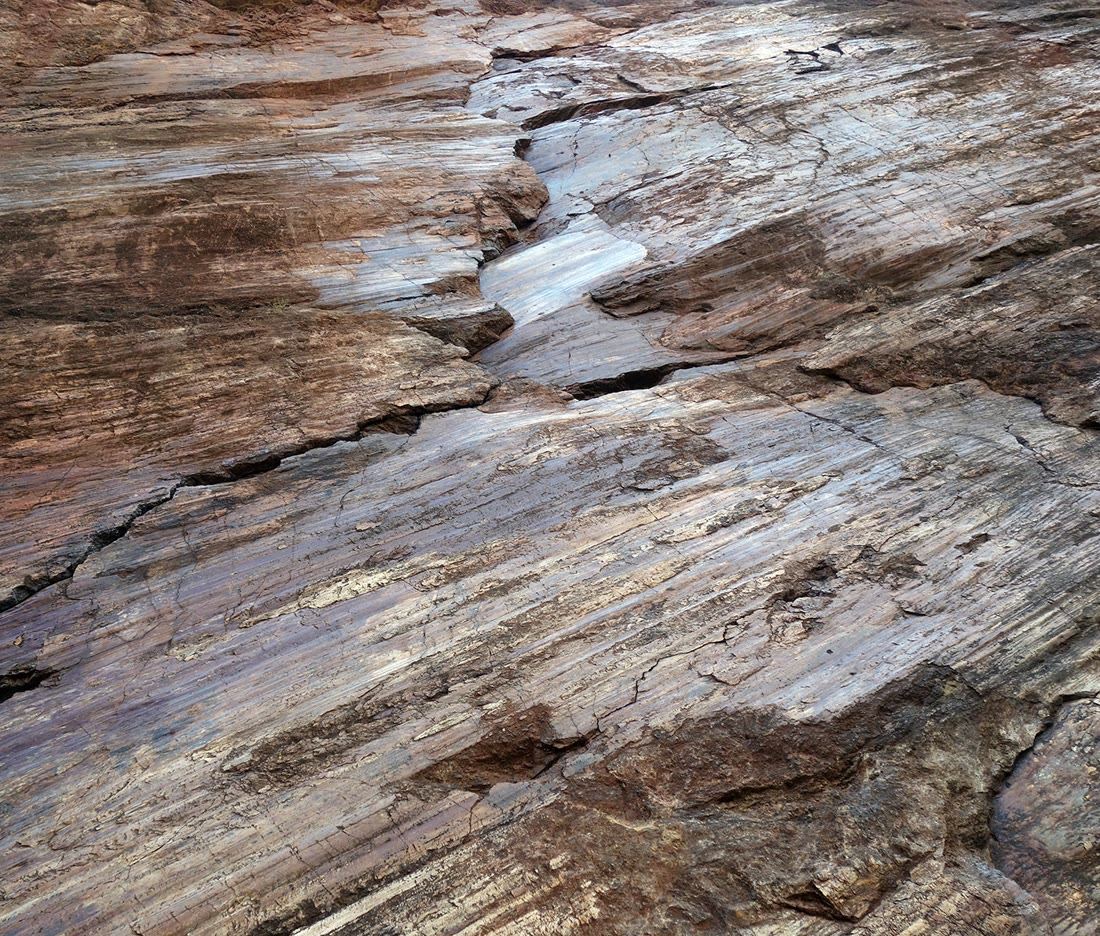
\includegraphics[height=5.2cm]{images/book3/b1-slickenside.jpg}\hfill
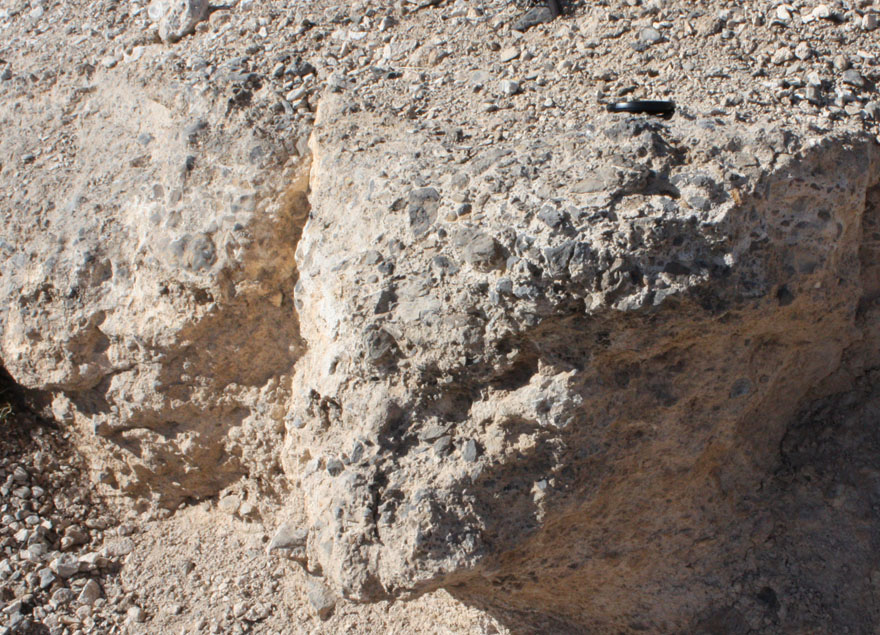
\includegraphics[height=5.2cm]{images/book3/b1-fault-breccia.jpg}
\par\smallskip{\small À esquerda: um \omterm{def:b1:faults-folds-fabrics:fault-rocks}{espelho de falha} em uma superfície de falha em sílex, de cerca de \qtyproduct{3 x 3}{m} de uma superfície de \qty{10}{m} de altura, Corona Heights, San Francisco; a face polida está estriada ao longo do deslizamento. Foto: Dextersinister, CC~BY-SA~4.0. À direita: \omterm{def:b1:faults-folds-fabrics:fault-rocks}{brecha de falha} da Keystone Thrust, Red Rock Canyon, Nevada: fragmentos angulosos de rocha carbonática cinza em uma matriz mais clara; a tampa da lente, no canto superior direito, tem \qty{5.8}{cm} de largura. Foto: Jstuby, domínio público. Ambas do Wikimedia Commons.}
\label{fig:b1:faults-folds-fabrics:fault-surfaces}
\end{omfigure}
% ledger: commons:slickenside, commons:breccia

\begin{method}[Medindo o deslizamento sobre uma falha]\label{met:b1:faults-folds-fabrics:slip}
\begin{enumerate}
  \item Meça a \omterm{def:b1:geological-maps:attitude}{atitude} $\alpha/\delta$ da superfície da falha e escreva sua \omterm{def:b1:geological-maps:attitude}{direção}, $\alpha - \ang{90}$.
  \item Meça as \omterm{def:b1:faults-folds-fabrics:fault-rocks}{estrias}: seu \omterm{def:b1:faults-folds-fabrics:fault-elements}{rake} na falha, ou seu \omterm{def:b1:field-lab-methods-1:trend-plunge}{rumo} e \omterm{def:b1:field-lab-methods-1:trend-plunge}{caimento}; para um \omterm{def:b1:faults-folds-fabrics:fault-elements}{rake} $r$, $\sin p = |\sin r|\sin\delta$.
  \item Descubra para que lado o \omterm{def:b1:faults-folds-fabrics:fault-elements}{bloco superior} se moveu, a partir de marcadores deslocados através da falha, e dê ao \omterm{def:b1:faults-folds-fabrics:fault-elements}{rake} seu sinal: negativo se o \omterm{def:b1:faults-folds-fabrics:fault-elements}{bloco superior} desceu.
  \item Encontre o \omterm{def:b1:faults-folds-fabrics:fault-elements}{deslizamento líquido} $L$ a partir de dois pontos que foram um só; se só o \omterm{def:b1:cross-sections:throw}{rejeito} vertical $h$ de um marcador horizontal é conhecido, $L = h/(|\sin r|\sin\delta)$.
  \item Calcule as componentes com
        \cref{prop:b1:faults-folds-fabrics:slip-components} e dê nome à falha com
        \cref{def:b1:faults-folds-fabrics:fault-types}.
\end{enumerate}
\end{method}

\begin{inthefield}[Medindo uma superfície de falha]
Um geólogo que encontra uma superfície de falha num \omterm{def:b1:geological-maps:geological-map}{afloramento} a mede como qualquer outro plano, com uma bússola-clinômetro apoiada sobre a superfície, e depois mede as \omterm{def:b1:faults-folds-fabrics:fault-rocks}{estrias} sobre ela, seja como \omterm{def:b1:faults-folds-fabrics:fault-elements}{rake}, com um transferidor apoiado no plano, seja como \omterm{def:b1:field-lab-methods-1:trend-plunge}{rumo} e \omterm{def:b1:field-lab-methods-1:trend-plunge}{caimento}. Os dois são conferidos um com o outro pela fórmula do passo 2 do método. O sentido do movimento é a parte difícil. Pequenos degraus em um \omterm{def:b1:faults-folds-fabrics:fault-rocks}{espelho de falha}, e fibras de quartzo ou calcita que cresceram à medida que os blocos se afastavam, podem mostrar para que lado o bloco faltante foi, mas alguns degraus apontam para o lado errado; por isso o sentido só é confiável quando concorda com o deslocamento de uma camada marcadora ou de um veio. As \omterm{def:b1:faults-folds-fabrics:fault-rocks}{rochas de falha} são descritas e amostradas, e uma zona de falha larga demais para ser medida em um só lugar é mapeada como uma faixa. Cada falha é registrada em uma estação numerada do caderno, com sua \omterm{def:b1:geological-maps:attitude}{atitude}, suas \omterm{def:b1:faults-folds-fabrics:fault-rocks}{estrias}, o sentido do movimento e quão seguro o geólogo está dele.
\end{inthefield}

\section{A teoria de Anderson das falhas}\label{sec:b1:faults-folds-fabrics:anderson}

Por que a maioria das falhas normais é íngreme e a maioria dos empurrões é suave? Em 1905, o geólogo escocês Ernest Masson Anderson respondeu com duas observações: a superfície da Terra fixa as direções das \omterm{def:b1:stress-strain-rheology:principal}{tensões principais}, e o critério de Coulomb então fixa o ângulo das falhas.
% ledger: ws:anderson, anderson:1905

\begin{proposition}[Uma superfície livre faz um plano principal]\label{prop:b1:faults-folds-fabrics:free-surface}
Na superfície da Terra, onde ela é horizontal, uma tensão principal é vertical e as outras duas são horizontais.
\end{proposition}

\begin{proof}
O ar pressiona o solo apenas com sua pressão, normal à superfície: não exerce tensão de cisalhamento. A tensão sobre o plano horizontal na superfície é portanto normal a ele. Em três dimensões, a tensão sobre um plano de normal unitária $\mathbf n$ é o vetor $\boldsymbol\sigma\mathbf n$ (livros de física, Livro 5); se ele não tem parte de cisalhamento, é paralelo a $\mathbf n$, de modo que
$\boldsymbol\sigma\mathbf n = \lambda\mathbf n$ e $\mathbf n$ é um autovetor da matriz simétrica $\boldsymbol\sigma$: uma direção principal (\cref{def:b1:stress-strain-rheology:principal}). A vertical é assim uma direção principal, e as outras duas, perpendiculares a ela, são horizontais.
\end{proof}

Anderson supôs que as \omterm{def:b1:stress-strain-rheology:principal}{tensões principais} mantêm essas direções até as profundidades em que se formam as falhas. A suposição vale bem sob uma superfície suavemente inclinada e em rochas sem fraquezas antigas fortes; ela falha perto de uma topografia íngreme e onde falhas ou camadas antigas guiam as novas. Com ela, só são possíveis três casos, conforme qual de $\sigma_1$, $\sigma_2$ e
$\sigma_3$ é vertical.

\begin{theorem}[Teoria de Anderson das falhas]\label{thm:b1:faults-folds-fabrics:anderson}
Seja uma tensão principal vertical, e rompa-se a rocha segundo o critério de Coulomb, com \omterm{def:b1:stress-strain-rheology:coulomb}{ângulo de atrito interno} $\phi$. Novas falhas se formam em planos que contêm a direção de $\sigma_2$ e fazem o ângulo $\ang{45} - \phi/2$ com $\sigma_1$, e deslizam perpendicularmente a $\sigma_2$, encurtando a rocha ao longo de $\sigma_1$. Daí
\begin{enumerate}[label=(\alph*)]
  \item se $\sigma_1$ é vertical, formam-se falhas normais, com \omterm{def:b1:geological-maps:attitude}{direção} ao longo de
        $\sigma_2$ e \omterm{def:b1:geological-maps:attitude}{mergulho} $\ang{45} + \phi/2$;
  \item se $\sigma_3$ é vertical, formam-se \omterm{def:b1:faults-folds-fabrics:fault-types}{falhas de empurrão}, com \omterm{def:b1:geological-maps:attitude}{direção} ao longo de
        $\sigma_2$ e \omterm{def:b1:geological-maps:attitude}{mergulho} $\ang{45} - \phi/2$;
  \item se $\sigma_2$ é vertical, formam-se \omterm{def:b1:faults-folds-fabrics:fault-types}{falhas transcorrentes} verticais, com \omterm{def:b1:geological-maps:attitude}{direção}
        formando $\ang{45} - \phi/2$ de cada lado de $\sigma_1$.
\end{enumerate}
Com $\phi = \ang{30}$, os \omterm{def:b1:geological-maps:attitude}{mergulhos} são \ang{60}, \ang{30} e \ang{90}.
\end{theorem}
\index{teoria de Anderson das falhas}

\begin{proof}
Num plano que contém a direção de $\sigma_2$, a normal jaz no plano de $\sigma_1$ e $\sigma_3$, e a tensão sobre o plano é a do problema bidimensional de
\cref{ch:b1:stress-strain-rheology}: seu ponto jaz sobre o círculo de Mohr de $\sigma_1$ e $\sigma_3$, e sua parte de cisalhamento jaz no plano de $\sigma_1$ e $\sigma_3$, perpendicular a $\sigma_2$.
Em qualquer outro plano, o ponto $(\sigma_n, \tau)$ jaz dentro desse círculo, que é o maior dos três círculos de Mohr de um estado de tensão tridimensional (admitido a partir da teoria tridimensional). À medida que as tensões crescem, a reta de Coulomb é portanto tocada primeiro pelos planos que contêm $\sigma_2$, e entre eles, pelo \cref{thm:b1:stress-strain-rheology:failure-angle}, pelos que fazem $\ang{45} - \phi/2$ com $\sigma_1$. O deslizamento sobre tal plano, perpendicular a $\sigma_2$, aproxima os dois blocos ao longo da \omterm{def:b1:geological-maps:attitude}{direção} de maior compressão e os afasta ao longo da menor, como deve para aliviar a tensão. No caso (a), o plano faz o ângulo $\ang{45} - \phi/2$ com a
vertical, logo mergulha $\ang{45} + \phi/2$; sua \omterm{def:b1:geological-maps:attitude}{direção} é a de $\sigma_2$, horizontal; o deslizamento jaz no plano vertical do \omterm{def:b1:geological-maps:attitude}{mergulho}, e o \omterm{def:b1:faults-folds-fabrics:fault-elements}{bloco superior} desce, alongando a rocha horizontalmente: uma \omterm{def:b1:faults-folds-fabrics:fault-types}{falha normal}. No caso (b), o plano faz $\ang{45} - \phi/2 < \ang{45}$ com o $\sigma_1$ horizontal, e o deslizamento encurta a rocha horizontalmente, empurrando o \omterm{def:b1:faults-folds-fabrics:fault-elements}{bloco superior} para cima: uma \omterm{def:b1:faults-folds-fabrics:fault-types}{falha de empurrão}. No caso (c), os planos contêm a vertical, logo são verticais; o deslizamento é horizontal, perpendicular a $\sigma_2$: \omterm{def:b1:faults-folds-fabrics:fault-types}{falhas transcorrentes}, a $\ang{45} - \phi/2$ de cada lado do $\sigma_1$ horizontal.
\end{proof}

Em cada regime são possíveis dois conjuntos de falhas, simétricos em torno de $\sigma_1$: falhas conjugadas, que se encontram em $\ang{90} - \phi$, cerca de \ang{60}, com $\sigma_1$ no ângulo agudo entre elas. Inversamente, um par de falhas conjugadas medido no campo dá as direções das tensões que as fizeram: $\sigma_1$ divide ao meio seu ângulo agudo, e $\sigma_2$ é sua linha de interseção.

\begin{omfigure}
\begin{tikzpicture}[x={(1cm,0cm)}, y={(0.42cm,0.30cm)}, z={(0cm,1cm)},
  >={Stealth[length=5pt]}, font=\small, scale=0.86,
  face/.style={draw=black, line width=0.5pt, line join=round},
  sone/.style={->, line width=1.6pt, omThm},
  sthree/.style={->, line width=0.8pt, omDef}]
% exact geometry: the fault plane is X = xf(Z); slip is along the dip; throw t
% (a) normal fault: dip 60, xf(Z) = 1.3 + (1.6 - Z)/tan 60, throw 0.45
\begin{scope}
  \def\W{3.2}\def\D{1.6}\def\H{1.6}
  \pgfmathsetmacro{\c}{1/tan(60)}
  \pgfmathsetmacro{\xa}{1.3+1.6*\c}       % xf(0)
  \pgfmathsetmacro{\xb}{1.3+0.45*\c}      % xf(H - t)
  \pgfmathsetmacro{\mfa}{1.3+(1.6-0.55)*\c}\pgfmathsetmacro{\mfb}{1.3+(1.6-0.85)*\c}
  \pgfmathsetmacro{\mha}{1.3+(1.6-0.10)*\c}\pgfmathsetmacro{\mhb}{1.3+(1.6-0.40)*\c}
  % footwall
  \fill[omLithSand!55] (0,0,0) -- (\xa,0,0) -- (1.3,0,\H) -- (0,0,\H) -- cycle;
  \fill[omProp!40] (0,0,0.55) -- (\mfa,0,0.55) -- (\mfb,0,0.85) -- (0,0,0.85) -- cycle;
  \draw[face] (0,0,0) -- (\xa,0,0) -- (1.3,0,\H) -- (0,0,\H) -- cycle;
  \draw[face, fill=omLithSand!35] (0,0,\H) -- (1.3,0,\H) -- (1.3,\D,\H) -- (0,\D,\H) -- cycle;
  \draw[face, fill=black!12] (1.3,0,\H) -- (\xb,0,1.15) -- (\xb,\D,1.15) -- (1.3,\D,\H) -- cycle;
  % hanging wall
  \fill[omLithSand!55] (\xa,0,0) -- (\W,0,0) -- (\W,0,1.15) -- (\xb,0,1.15) -- cycle;
  \fill[omProp!40] (\mha,0,0.10) -- (\W,0,0.10) -- (\W,0,0.40) -- (\mhb,0,0.40) -- cycle;
  \draw[face] (\xa,0,0) -- (\W,0,0) -- (\W,0,1.15) -- (\xb,0,1.15) -- cycle;
  \draw[face, fill=omLithSand!35] (\xb,0,1.15) -- (\W,0,1.15) -- (\W,\D,1.15) -- (\xb,\D,1.15) -- cycle;
  \fill[omLithSand!45] (\W,0,0) -- (\W,\D,0) -- (\W,\D,1.15) -- (\W,0,1.15) -- cycle;
  \fill[omProp!30] (\W,0,0.10) -- (\W,\D,0.10) -- (\W,\D,0.40) -- (\W,0,0.40) -- cycle;
  \draw[face] (\W,0,0) -- (\W,\D,0) -- (\W,\D,1.15) -- (\W,0,1.15) -- cycle;
  % slip arrow on the front face
  \draw[->, line width=0.9pt] (1.45,0,1.05) -- ++({0.35*cos(60)},0,{-0.35*sin(60)});
  % stresses: sigma1 vertical, sigma3 horizontal across the strike
  \draw[sone] (1.6,0.8,3.05) -- (1.6,0.8,2.1) node[pos=0, left] {$\sigma_1$};
  \draw[sone] (1.6,0.8,-1.1) -- (1.6,0.8,-0.15);
  \draw[sthree] (-0.85,0.8,0.8) -- (-0.15,0.8,0.8) node[pos=0, above] {$\sigma_3$};
  \draw[sthree] (4.05,0.8,0.6) -- (3.35,0.8,0.6);
  \node[font=\small\bfseries] at (1.9,0,-1.55) {(a) falha normal};
\end{scope}
% (b) thrust fault: dip 30, xf(Z) = 3.0 - Z/tan 30, throw 0.35, heave 0.606
\begin{scope}[xshift=6.0cm]
  \def\D{1.6}\def\H{1.3}
  \pgfmathsetmacro{\c}{1/tan(30)}
  \pgfmathsetmacro{\Wp}{4.0-0.35*\c}       % right face of the hanging wall
  \pgfmathsetmacro{\xt}{3.0-1.3*\c}        % footwall top edge
  \pgfmathsetmacro{\xh}{3.0-1.65*\c}       % hanging-wall top edge
  \pgfmathsetmacro{\mfa}{3.0-0.50*\c}\pgfmathsetmacro{\mfb}{3.0-0.75*\c}
  \pgfmathsetmacro{\mha}{3.0-0.85*\c}\pgfmathsetmacro{\mhb}{3.0-1.10*\c}
  % footwall
  \fill[omLithSand!55] (0,0,0) -- (3.0,0,0) -- (\xt,0,\H) -- (0,0,\H) -- cycle;
  \fill[omProp!40] (0,0,0.50) -- (\mfa,0,0.50) -- (\mfb,0,0.75) -- (0,0,0.75) -- cycle;
  \draw[face] (0,0,0) -- (3.0,0,0) -- (\xt,0,\H) -- (0,0,\H) -- cycle;
  \draw[face, fill=omLithSand!35] (0,0,\H) -- (\xt,0,\H) -- (\xt,\D,\H) -- (0,\D,\H) -- cycle;
  % hanging wall
  \fill[omLithSand!55] (3.0,0,0) -- (\Wp,0,0) -- (\Wp,0,1.65) -- (\xh,0,1.65) -- cycle;
  \fill[omProp!40] (\mha,0,0.85) -- (\Wp,0,0.85) -- (\Wp,0,1.10) -- (\mhb,0,1.10) -- cycle;
  \draw[face] (3.0,0,0) -- (\Wp,0,0) -- (\Wp,0,1.65) -- (\xh,0,1.65) -- cycle;
  \draw[face, fill=omLithSand!35] (\xh,0,1.65) -- (\Wp,0,1.65) -- (\Wp,\D,1.65) -- (\xh,\D,1.65) -- cycle;
  \fill[omLithSand!45] (\Wp,0,0) -- (\Wp,\D,0) -- (\Wp,\D,1.65) -- (\Wp,0,1.65) -- cycle;
  \fill[omProp!30] (\Wp,0,0.85) -- (\Wp,\D,0.85) -- (\Wp,\D,1.10) -- (\Wp,0,1.10) -- cycle;
  \draw[face] (\Wp,0,0) -- (\Wp,\D,0) -- (\Wp,\D,1.65) -- (\Wp,0,1.65) -- cycle;
  \draw[->, line width=0.9pt] (2.25,0,0.62) -- ++({-0.42*cos(30)},0,{0.42*sin(30)});
  % stresses: sigma1 horizontal across the strike, sigma3 vertical
  \draw[sone] (-1.2,0.8,0.65) -- (-0.15,0.8,0.65) node[pos=0, above] {$\sigma_1$};
  \draw[sone] (\Wp+1.15,0.8,0.45) -- (\Wp+0.1,0.8,0.45);
  \draw[sthree] (2.0,0.8,2.7) -- (2.0,0.8,2.0) node[pos=0, left] {$\sigma_3$};
  \draw[sthree] (2.0,0.8,-0.9) -- (2.0,0.8,-0.2);
  \node[font=\small\bfseries] at (2.0,0,-1.55) {(b) falha de empurrão};
\end{scope}
% (c) strike-slip fault: vertical, along the y axis at X = 1.6; dextral: the far
% (east) block has moved toward the reader by 0.5; sigma1 at 30 deg clockwise of the strike
\begin{scope}[xshift=12.0cm]
  \def\D{2.2}\def\H{1.1}\def\s{0.5}
  % west block
  \draw[face, fill=omLithSand!55] (0,0,0) -- (1.6,0,0) -- (1.6,0,\H) -- (0,0,\H) -- cycle;
  \draw[face, fill=omLithSand!35] (0,0,\H) -- (1.6,0,\H) -- (1.6,\D,\H) -- (0,\D,\H) -- cycle;
  \draw[face, fill=black!12] (1.6,\D-\s,0) -- (1.6,\D,0) -- (1.6,\D,\H) -- (1.6,\D-\s,\H) -- cycle;
  \draw[line width=1.4pt, omProp] (0,1.25,\H) -- (1.6,1.25,\H);
  % east block
  \draw[face, fill=omLithSand!55] (1.6,-\s,0) -- (3.2,-\s,0) -- (3.2,-\s,\H) -- (1.6,-\s,\H) -- cycle;
  \draw[face, fill=omLithSand!35] (1.6,-\s,\H) -- (3.2,-\s,\H) -- (3.2,\D-\s,\H) -- (1.6,\D-\s,\H) -- cycle;
  \draw[face, fill=omLithSand!45] (3.2,-\s,0) -- (3.2,\D-\s,0) -- (3.2,\D-\s,\H) -- (3.2,-\s,\H) -- cycle;
  \draw[line width=1.4pt, omProp] (1.6,1.25-\s,\H) -- (3.2,1.25-\s,\H);
  % slip arrows on the top
  \draw[->, line width=0.9pt] (2.05,1.35,\H) -- (2.05,0.35,\H);
  \draw[->, line width=0.9pt] (1.15,0.55,\H) -- (1.15,1.55,\H);
  % stresses in the horizontal plane, drawn at the height of the top surface
  \draw[sone] ({1.6+1.9*sin(30)},{0.8+1.9*cos(30)},\H) -- ({1.6+1.0*sin(30)},{0.8+1.0*cos(30)},\H) node[pos=0, right] {$\sigma_1$};
  \draw[sone] ({1.6-1.9*sin(30)},{0.8-1.9*cos(30)},\H) -- ({1.6-1.0*sin(30)},{0.8-1.0*cos(30)},\H);
  \draw[sthree] ({1.6+2.0*sin(120)},{0.8+2.0*cos(120)},\H) -- ({1.6+1.45*sin(120)},{0.8+1.45*cos(120)},\H) node[pos=0, right] {$\sigma_3$};
  \draw[sthree] ({1.6-2.0*sin(120)},{0.8-2.0*cos(120)},\H) -- ({1.6-1.45*sin(120)},{0.8-1.45*cos(120)},\H);
  \node[font=\small\bfseries] at (1.7,0,-1.55) {(c) falha transcorrente};
\end{scope}
\end{tikzpicture}
\par\smallskip{\small Os três regimes de Anderson, com as falhas nos \omterm{def:b1:geological-maps:attitude}{mergulhos} do teorema para $\phi = \ang{30}$: \ang{60}, \ang{30} e vertical. Setas vermelhas grossas: $\sigma_1$; setas azuis finas: $\sigma_3$; $\sigma_2$ corre ao longo da \omterm{def:b1:geological-maps:attitude}{direção} das falhas em (a) e (b) e é vertical em (c). Um marcador (laranja) é deslocado pelo \omterm{def:b1:cross-sections:throw}{rejeito} em (a) e (b); em (c) uma linha no solo é deslocada horizontalmente, e a falha é \omterm{def:b1:faults-folds-fabrics:fault-types}{dextral}: visto de qualquer bloco, o outro se moveu para a direita. As setas pretas dão o deslizamento.}
\label{fig:b1:faults-folds-fabrics:anderson}
\end{omfigure}

Os três regimes correspondem aos três tipos de limite de placa descritos em
\cref{ch:b1:rifts-ridges-margins,ch:b1:active-margins}.
Onde a \omterm{def:b1:layered-earth:lithosphere}{litosfera} é distendida, em riftes e dorsais, a tensão horizontal fica abaixo da vertical e formam-se falhas normais; onde é comprimida, em limites convergentes e em cinturões de montanhas, a tensão horizontal excede o peso da rocha e formam-se empurrões; ao longo de \omterm{def:b1:rifts-ridges-margins:transform}{falhas transformantes}, as duas tensões horizontais envolvem a vertical. Os \omterm{def:b1:geological-maps:attitude}{mergulhos} se ajustam às observações de modo grosseiro: as falhas normais dos riftes mergulham cerca de \ang{60} perto da superfície, e os empurrões são \omterm{def:b1:faults-folds-fabrics:fault-types}{falhas inversas} de baixo ângulo.
O que não se encaixa é instrutivo. Muitas falhas normais se achatam com a profundidade, e algumas seções de riftes as mostram chegando a uma zona de cisalhamento quase plana: essas falhas de baixo ângulo, ou descolamentos, cortam a \omterm{def:b1:layered-earth:layers}{crosta} a bem menos de \ang{45}. A teoria de Anderson não consegue explicá-las como falhas novas, e o \cref{exo:b1:faults-folds-fabrics:10} mostra que o atrito de Byerlee tampouco consegue fazê-las deslizar sob tensões andersonianas: elas precisam de \omterm{def:b1:faults-folds-fabrics:fault-rocks}{rochas de falha} fracas, de pressão alta nos poros ou de tensões giradas.
Uma falha que já existe desliza com o atrito da \omterm{prop:b1:stress-strain-rheology:byerlee}{lei de Byerlee}, $\mu = 0.85$, $\phi = \ang{40.4}$; as falhas normais mais bem orientadas então mergulham \ang{65.2}, como mostrou o problema do \cref{ch:b1:stress-strain-rheology}.
% ledger: ws:anderson, usgs:fault-types, byerlee:1975

\begin{history}[Falhas de Anderson]
Ernest Masson Anderson, geólogo escocês, publicou sua teoria dos três tipos de falhas em 1905, em um artigo curto sobre a dinâmica do falhamento, e deu sua forma completa, com sua aplicação aos diques e falhas da Grã-Bretanha, em seu livro \emph{The Dynamics of Faulting and Dyke Formation}. Um pequeno número de artigos e esse livro ainda moldam a geologia estrutural, a sismologia e a mecânica das rochas: seus três regimes, normal, de empurrão e transcorrente, são o modo usual de classificar os estados de tensão da \omterm{def:b1:layered-earth:layers}{crosta} e as falhas que eles produzem, e de ler a tensão a partir das falhas.
\end{history}
% ledger: anderson:1905, healy:anderson, ws:anderson

\section{Geometria das dobras}\label{sec:b1:faults-folds-fabrics:folds}

\Cref{ch:b1:geological-maps} nomeou \omterm{def:b1:geological-maps:fold}{dobras} e leu seus padrões em mapas. Em três dimensões, uma \omterm{def:b1:geological-maps:fold}{dobra} precisa de mais nomes: onde ela se curva, com que agudeza, e como está posta no espaço.

\begin{definition}[Charneira, linha de charneira, flanco, plano axial, ângulo entre flancos, dobra cilíndrica]\label{def:b1:faults-folds-fabrics:fold-elements}
Sobre uma superfície dobrada, a \emph{charneira}\index{charneira (de uma dobra)} é a zona de maior curvatura, e a \emph{linha de charneira}\index{linha de charneira} a linha que une seus pontos de maior curvatura; os \emph{flancos}\index{flanco (de uma dobra)} são as partes menos curvas de cada lado. A superfície axial de uma \omterm{def:b1:geological-maps:fold}{dobra} é a superfície que une as linhas de charneira de suas superfícies dobradas sucessivas; quando é um plano, é o \emph{plano axial}\index{plano axial}. O \emph{ângulo entre flancos}\index{ângulo entre flancos} $\iota$ é o ângulo entre os dois flancos, medido no perfil, no plano perpendicular à linha de charneira, entre as tangentes aos flancos em seus pontos de inflexão; $0 \le \iota \le \ang{180}$. Uma \omterm{def:b1:geological-maps:fold}{dobra} é uma \emph{dobra cilíndrica}\index{dobra cilíndrica} quando suas superfícies são geradas por uma reta movida paralelamente a si mesma; a \omterm{def:b1:geological-maps:attitude}{direção} dessa reta é o eixo da \omterm{def:b1:geological-maps:fold}{dobra} de \cref{def:b1:geological-maps:fold}, e toda linha de charneira de uma \omterm{def:b1:geological-maps:fold}{dobra} cilíndrica é uma reta paralela a ele.
\end{definition}
% ledger: ws:fold-elements

\begin{omfigure}
\begin{tikzpicture}[x={(1cm,0cm)}, y={(0.42cm,0.30cm)}, z={(0cm,1cm)},
  >={Stealth[length=5pt]}, font=\small, scale=1.15]
% a cylindrical anticline: the top of a bed is z = f(x) = 0.35 a - a sqrt(x^2 + 0.35^2), a = tan 50
% (limbs dip toward 50 deg, interlimb angle 80 deg); the bed is 0.7 thick, measured vertically
% (a similar fold); the fold axis is the y direction, horizontal.
\def\D{2.8}
\pgfmathsetmacro{\a}{tan(50)}
\def\f(#1){0.35*\a - \a*sqrt((#1)*(#1) + 0.1225)}
\pgfmathsetmacro{\zt}{0.35*\a}
% top surface of the bed
\fill[omLithSand!35] plot[domain=-1.7:1.7, samples=61, variable=\x] (\x, 0, {\f(\x)})
  -- plot[domain=1.7:-1.7, samples=61, variable=\x] (\x, \D, {\f(\x)}) -- cycle;
\foreach \u in {-1.4,-1.0,-0.6,-0.3,0.3,0.6,1.0,1.4} {
  \draw[black!35, line width=0.3pt] (\u, 0, {\f(\u)}) -- (\u, \D, {\f(\u)});
}
\draw[line width=0.5pt] plot[domain=-1.7:1.7, samples=61, variable=\x] (\x, \D, {\f(\x)});
\draw[line width=0.5pt] (-1.7, 0, {\f(-1.7)}) -- (-1.7, \D, {\f(-1.7)});
% right end face
\fill[omLithSand!55] (1.7, 0, {\f(1.7)}) -- (1.7, \D, {\f(1.7)}) -- (1.7, \D, {\f(1.7)-0.7}) -- (1.7, 0, {\f(1.7)-0.7}) -- cycle;
\draw[line width=0.5pt] (1.7, 0, {\f(1.7)}) -- (1.7, \D, {\f(1.7)}) -- (1.7, \D, {\f(1.7)-0.7}) -- (1.7, 0, {\f(1.7)-0.7});
% axial plane, behind the front face
\fill[omDef!30, opacity=0.5] (0, 0, 0.85) -- (0, \D, 0.85) -- (0, \D, -2.0) -- (0, 0, -2.0) -- cycle;
\draw[omDef, line width=0.6pt] (0, 0, -2.0) -- (0, 0, 0.85) -- (0, \D, 0.85) -- (0, \D, -2.0);
% hinge line
\draw[omThm, line width=1.5pt] (0, 0, 0) -- (0, \D, 0);
% front face of the bed (the profile)
\fill[omLithSand!80] plot[domain=-1.7:1.7, samples=61, variable=\x] (\x, 0, {\f(\x)})
  -- plot[domain=1.7:-1.7, samples=61, variable=\x] (\x, 0, {\f(\x)-0.7}) -- cycle;
\draw[line width=0.7pt] plot[domain=-1.7:1.7, samples=61, variable=\x] (\x, 0, {\f(\x)});
\draw[line width=0.7pt] plot[domain=-1.7:1.7, samples=61, variable=\x] (\x, 0, {\f(\x)-0.7});
\draw[line width=0.5pt] (-1.7, 0, {\f(-1.7)}) -- (-1.7, 0, {\f(-1.7)-0.7});
\draw[omDef, line width=0.6pt, dashed] (0, 0, 0) -- (0, 0, -0.7);
\draw[omDef, line width=0.6pt] (0, 0, -0.7) -- (0, 0, -2.0);
% interlimb angle on the profile, in the core: tangents to the limbs of the base of the bed
% meet at (0, 0, zt - 0.7)
\pgfmathsetmacro{\zb}{\zt-0.7}
\draw[black!70, dashed] (-1.3, 0, {\zb-1.3*\a}) -- (0, 0, \zb) -- (1.3, 0, {\zb-1.3*\a});
\draw[black, line width=0.5pt] plot[domain=-140:-40, samples=21, variable=\t] ({0.75*cos(\t)}, 0, {\zb+0.75*sin(\t)});
\node[font=\scriptsize] at (0.22, 0, {\zb-1.0}) {$\iota$};
% labels
\node[omThm, anchor=west, font=\scriptsize] at (0.08, \D, 0.1) {linha de charneira};
\node[omDef, anchor=south, font=\scriptsize] at (0, \D, 0.85) {plano axial};
\node[font=\scriptsize, rotate=50] at (-1.15, 0, {\f(-1.15)-0.35}) {flanco};
\node[font=\scriptsize, rotate=-50] at (1.15, 0, {\f(1.15)-0.35}) {flanco};
\end{tikzpicture}
\par\smallskip{\small Os elementos de um \omterm{def:b1:geological-maps:fold}{anticlinal} cilíndrico, aqui com uma \omterm{def:b1:faults-folds-fabrics:fold-elements}{linha de charneira} horizontal: a \omterm{def:b1:faults-folds-fabrics:fold-elements}{charneira}, onde a camada mais se curva; os dois \omterm{def:b1:faults-folds-fabrics:fold-elements}{flancos}; o \omterm{def:b1:faults-folds-fabrics:fold-elements}{plano axial} pelas \omterm{def:b1:faults-folds-fabrics:fold-elements}{linhas de charneira} do topo e da base da camada; e o \omterm{def:b1:faults-folds-fabrics:fold-elements}{ângulo entre flancos} $\iota$ entre as tangentes aos \omterm{def:b1:faults-folds-fabrics:fold-elements}{flancos}, medido no perfil da frente, aqui \ang{80}, desenhado na base da camada. As linhas cinzas sobre o topo da camada são paralelas ao eixo da \omterm{def:b1:geological-maps:fold}{dobra}.}
\label{fig:b1:faults-folds-fabrics:fold-elements}
\end{omfigure}

Quando os \omterm{def:b1:faults-folds-fabrics:fold-elements}{flancos} são planos, como nas \omterm{def:b1:geological-maps:fold}{dobras} em chevron abaixo e nas Colinas de Varden, a geometria de uma \omterm{def:b1:geological-maps:fold}{dobra} decorre das \omterm{def:b1:geological-maps:attitude}{atitudes} de seus \omterm{def:b1:faults-folds-fabrics:fold-elements}{flancos}. A normal unitária ascendente de um plano de \omterm{def:b1:geological-maps:attitude}{sentido de mergulho} $\alpha$ e \omterm{def:b1:geological-maps:attitude}{mergulho} $\delta$ é
$\mathbf n = (\sin\delta\sin\alpha, \sin\delta\cos\alpha, \cos\delta)$, em componentes leste, norte e para cima.

\begin{proposition}[Uma dobra a partir de seus flancos]\label{prop:b1:faults-folds-fabrics:hinge}
Seja uma \omterm{def:b1:faults-folds-fabrics:fold-elements}{dobra cilíndrica} de \omterm{def:b1:faults-folds-fabrics:fold-elements}{flancos} planos, nenhum invertido, com normais unitárias ascendentes $\mathbf n_1$ e $\mathbf n_2$. Sua \omterm{def:b1:faults-folds-fabrics:fold-elements}{linha de charneira} é paralela a
$\mathbf n_1 \times \mathbf n_2$, e seu \omterm{def:b1:faults-folds-fabrics:fold-elements}{ângulo entre flancos} é
\[
  \iota = \ang{180} - \arccos(\mathbf n_1\cdot\mathbf n_2) .
\]
\end{proposition}

\begin{proof}
Cada flanco é gerado por retas paralelas ao eixo da \omterm{def:b1:geological-maps:fold}{dobra}, logo contém a \omterm{def:b1:geological-maps:attitude}{direção} do eixo, que é portanto perpendicular às duas normais e paralelo a seu produto vetorial; a \omterm{def:b1:faults-folds-fabrics:fold-elements}{linha de charneira} é paralela ao eixo. O perfil é perpendicular ao eixo, logo contém as duas normais; nele, os dois \omterm{def:b1:faults-folds-fabrics:fold-elements}{flancos} aparecem como duas retas perpendiculares a $\mathbf n_1$ e $\mathbf n_2$, e o ângulo entre as retas é igual ao ângulo $\arccos(\mathbf n_1\cdot\mathbf n_2)$ entre as normais, ou a seu suplemento. Quando as camadas não estão dobradas, as duas normais coincidem e o \omterm{def:b1:faults-folds-fabrics:fold-elements}{ângulo entre flancos} é \ang{180}; à medida que os \omterm{def:b1:faults-folds-fabrics:fold-elements}{flancos} giram, o ângulo entre as normais cresce a partir de $0$ enquanto o \omterm{def:b1:faults-folds-fabrics:fold-elements}{ângulo entre flancos} diminui a partir de \ang{180}, de modo que os dois somam \ang{180} enquanto ambas as normais apontam para cima.
\end{proof}

Para uma \omterm{def:b1:faults-folds-fabrics:fold-classes}{dobra vertical} cujos dois \omterm{def:b1:faults-folds-fabrics:fold-elements}{flancos} mergulham $\delta$ para cada lado, as normais
fazem o ângulo $2\delta$ e $\iota = \ang{180} - 2\delta$.

\begin{definition}[Classes de dobras]\label{def:b1:faults-folds-fabrics:fold-classes}
Pelo seu \omterm{def:b1:faults-folds-fabrics:fold-elements}{ângulo entre flancos}, uma \omterm{def:b1:geological-maps:fold}{dobra} é uma \emph{dobra suave}\index{dobra suave} ($\iota$ de \ang{180} a \ang{170}), uma \emph{dobra aberta}\index{dobra aberta} (de \ang{170} a \ang{90}), uma \emph{dobra fechada}\index{dobra fechada} (de \ang{90} a
\ang{10}) ou, quando seus \omterm{def:b1:faults-folds-fabrics:fold-elements}{flancos} são quase paralelos ($\iota$ de \ang{10} a $0$), uma \emph{dobra isoclinal}\index{dobra isoclinal}. Pelo \omterm{def:b1:geological-maps:attitude}{mergulho} de seu \omterm{def:b1:faults-folds-fabrics:fold-elements}{plano axial}, uma \omterm{def:b1:geological-maps:fold}{dobra} é uma \emph{dobra vertical}\index{dobra vertical} quando o \omterm{def:b1:faults-folds-fabrics:fold-elements}{plano axial} mergulha mais que \ang{80}, uma \emph{dobra deitada}\index{dobra deitada} quando mergulha menos que \ang{10}, e uma \emph{dobra inclinada}\index{dobra inclinada} entre esses valores. Uma \omterm{def:b1:geological-maps:fold}{dobra} cujo flanco passou da vertical, de modo que ambos os \omterm{def:b1:faults-folds-fabrics:fold-elements}{flancos} mergulham para o mesmo lado e as camadas daquele flanco estão de cabeça para baixo, é uma \emph{dobra invertida}\index{dobra invertida}. Uma \omterm{def:b1:geological-maps:fold}{dobra} cuja \omterm{def:b1:faults-folds-fabrics:fold-elements}{linha de charneira} não é horizontal é uma \emph{dobra com caimento}\index{dobra com caimento}.
\end{definition}
Outros limites são usados para as classes de aperto; este livro mantém as quatro acima.
% ledger: ws:fold-classes, ws:fold-elements

\begin{omfigure}
\begin{tikzpicture}[font=\small]
% one antiform profile: a hinge arc of radius 0.22 and two straight limbs of length 1.05,
% each at half the interlimb angle (#1 = iota/2) from the downward axial trace; three
% surfaces repeated by a shift of 0.3 along the axial trace (a similar fold)
\newcommand{\foldprof}[2]{%
  \foreach \k in {0,1,2} {
    \draw[line width=0.7pt, #2]
      ($(0,-0.3*\k)+(180-#1:0.22)+({-1.05*sin(#1)},{-1.05*cos(#1)})$)
      -- ($(0,-0.3*\k)+(180-#1:0.22)$)
      arc[start angle=180-#1, end angle=#1, radius=0.22]
      -- ++({1.05*sin(#1)},{-1.05*cos(#1)});
  }
}
% row 1: tightness (the axial plane vertical)
\foreach \i/\n/\x in {174/suave/1.5, 120/aberta/4.5, 50/fechada/7.5, 0/isoclinal/10.5} {
  \begin{scope}[xshift=\x cm]
    \pgfmathsetmacro{\b}{\i/2}
    \draw[omDef, dashed, line width=0.5pt] (0,0.45) -- (0,-1.85);
    \foldprof{\b}{black}
    \node[font=\small\bfseries] at (0,-2.2) {\n};
    \node[font=\scriptsize] at (0,-2.6) {$\iota = \ang{\i}$};
  \end{scope}
}
% row 2: attitude of the axial plane (iota = 40 deg)
\foreach \d/\n/\x in {90/vertical/1.5, 50/inclinada/6.0, 8/deitada/10.5} {
  \begin{scope}[xshift=\x cm, yshift=-4.3cm]
    \begin{scope}[rotate={-(90-\d)}]
      \draw[omDef, dashed, line width=0.5pt] (0,0.55) -- (0,-1.85);
      \foldprof{20}{black}
    \end{scope}
    \node[font=\small\bfseries] at (0,-2.2) {\n};
    \node[font=\scriptsize] at (0,-2.6) {plano axial com mergulho de \ang{\d}};
  \end{scope}
}
\end{tikzpicture}
\par\smallskip{\small Classes de \omterm{def:b1:geological-maps:fold}{dobras}, em perfil. Em cima: pelo \omterm{def:b1:faults-folds-fabrics:fold-elements}{ângulo entre flancos}, com \omterm{def:b1:faults-folds-fabrics:fold-elements}{plano axial} vertical (tracejado). Embaixo: pelo \omterm{def:b1:geological-maps:attitude}{mergulho} do \omterm{def:b1:faults-folds-fabrics:fold-elements}{plano axial}, para \omterm{def:b1:geological-maps:fold}{dobras} de \omterm{def:b1:faults-folds-fabrics:fold-elements}{ângulo entre flancos} \ang{40}; a \omterm{def:b1:faults-folds-fabrics:fold-classes}{dobra inclinada} desenhada também está invertida, com seus dois \omterm{def:b1:faults-folds-fabrics:fold-elements}{flancos} mergulhando para a esquerda.}
\label{fig:b1:faults-folds-fabrics:classes}
\end{omfigure}

A espessura das camadas distingue dois estilos. Em \omterm{def:b1:geological-maps:fold}{dobras} paralelas, ou concêntricas, cada camada conserva sua espessura medida perpendicularmente a ela, como uma pilha de folhas de papel ao ser dobrada; tais \omterm{def:b1:geological-maps:fold}{dobras} se formam por flambagem de camadas fortes intercaladas com camadas muito fracas. Em \omterm{def:b1:geological-maps:fold}{dobras} semelhantes, cada superfície tem a mesma forma, as camadas conservam sua espessura medida paralelamente ao \omterm{def:b1:faults-folds-fabrics:fold-elements}{plano axial}, e afinam nos \omterm{def:b1:faults-folds-fabrics:fold-elements}{flancos} e engrossam nas \omterm{def:b1:faults-folds-fabrics:fold-elements}{charneiras}, como os perfis desenhados acima mostram; elas se formam quando todas as camadas são fracas, de modo que não desempenham papel mecânico. \omterm{def:b1:geological-maps:fold}{Dobras} em chevron têm \omterm{def:b1:faults-folds-fabrics:fold-elements}{flancos} retos e \omterm{def:b1:faults-folds-fabrics:fold-elements}{charneiras} estreitas, com um \omterm{def:b1:faults-folds-fabrics:fold-elements}{ângulo entre flancos} perto de \ang{60}; são \omterm{def:b1:geological-maps:fold}{dobras} paralelas de camadas fortes dispostas próximas umas das outras, que deslizam umas sobre as outras à medida que se dobram.
% ledger: ws:fold-elements

\begin{omfigure}
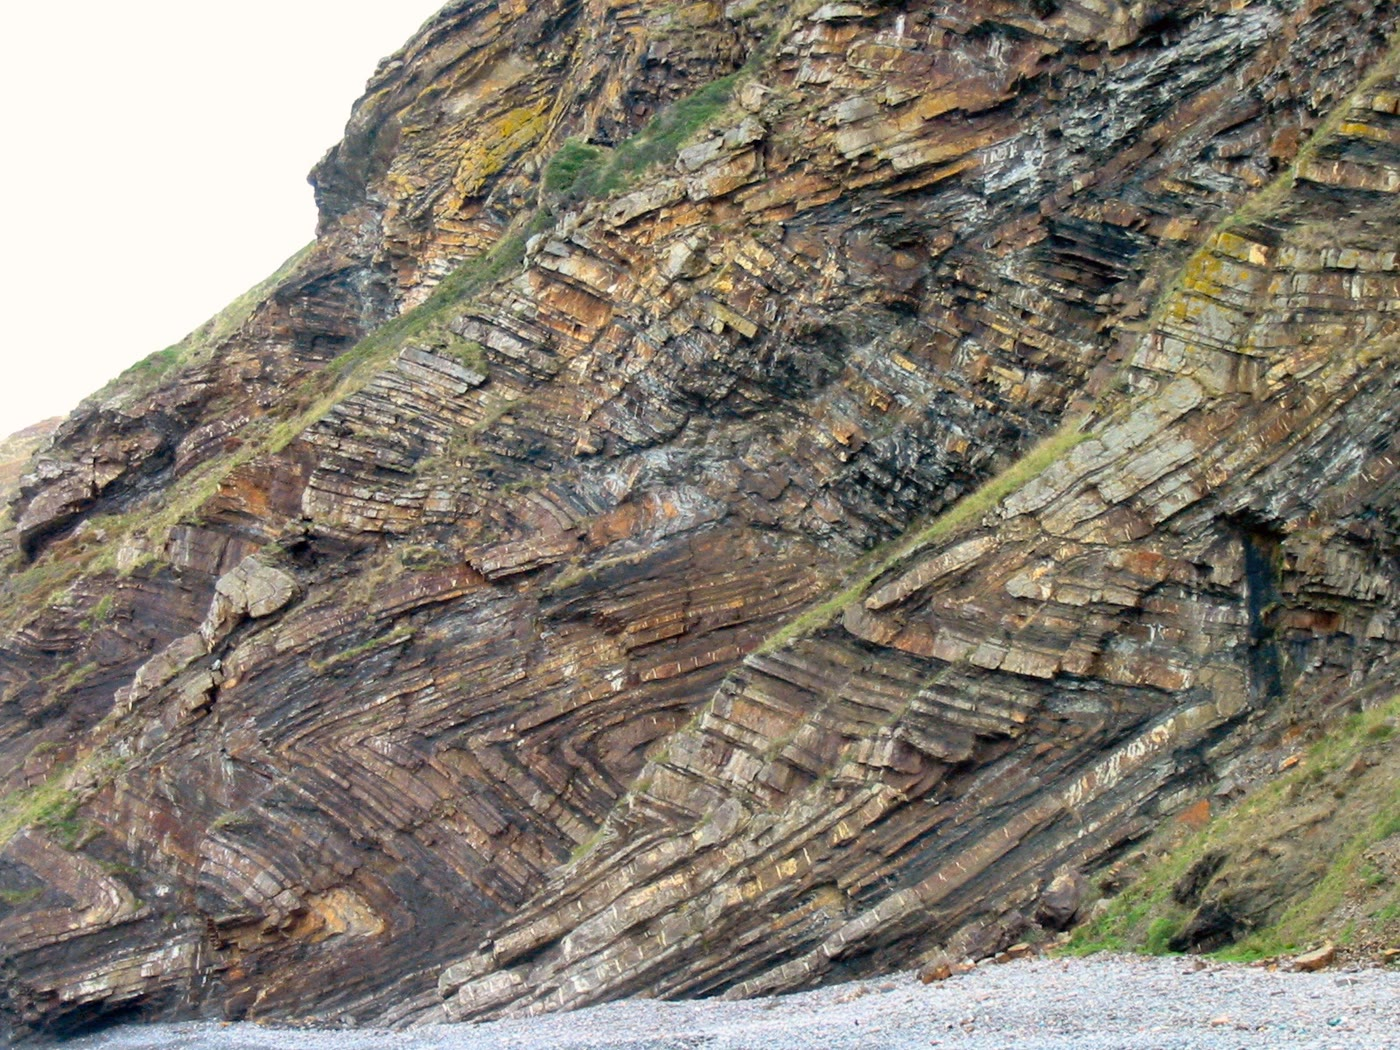
\includegraphics[width=0.78\linewidth]{images/book3/b1-chevron-folds-millook.jpg}
\par\smallskip{\small Camadas dobradas de arenito e folhelho nos penhascos de Millook, Cornualha do Norte: \omterm{def:b1:geological-maps:fold}{dobras} em chevron com \omterm{def:b1:faults-folds-fabrics:fold-elements}{flancos} quase retos e \omterm{def:b1:faults-folds-fabrics:fold-elements}{charneiras} agudas, com planos axiais quase verticais. Foto: Smalljim, CC~BY~3.0 (Wikimedia Commons).}
\label{fig:b1:faults-folds-fabrics:chevrons}
\end{omfigure}
% ledger: commons:millook

\section{Fábricas}\label{sec:b1:faults-folds-fabrics:fabrics}

Uma rocha deformada muitas vezes o é em toda a sua extensão, e não apenas em algumas superfícies: seus grãos são achatados, girados ou recristalizados em uma orientação comum, o que lhe dá uma fábrica. Uma fábrica planar faz a rocha se partir em lâminas; uma linear faz com que ela se parta em bastões.

\begin{definition}[Foliação, xistosidade, clivagem ardosiana, clivagem plano-axial]\label{def:b1:faults-folds-fabrics:foliation}
Uma \emph{foliação}\index{foliação} é uma fábrica planar que permeia uma rocha:
um conjunto de superfícies paralelas bem espaçadas, feitas por grãos achatados ou em placas alinhados ou por camadas finas, ao longo das quais a rocha se parte com mais facilidade.
\emph{Xistosidade}\index{xistosidade} é a foliação de um xisto, feita por grãos alinhados mais grossos que cerca de \qty{1}{mm}. Uma \emph{clivagem}\index{clivagem (de uma rocha)} é uma foliação de uma rocha de granulação fina feita por sua deformação; a \emph{clivagem ardosiana}\index{clivagem ardosiana} é a clivagem de uma ardósia, feita por \omterm{def:b1:rock-forming-minerals:silicate-classes}{filossilicatos} pequenos demais para serem vistos a olho nu, e tão próximos que a rocha pode ser partida quase em qualquer lugar em lâminas finas. Uma \emph{clivagem plano-axial}\index{clivagem plano-axial} é uma clivagem paralela, ou quase paralela, aos planos axiais das \omterm{def:b1:geological-maps:fold}{dobras} das mesmas rochas.
\end{definition}
% ledger: ws:fabrics

A \omterm{def:b1:faults-folds-fabrics:foliation}{foliação} forma-se aproximadamente perpendicular à \omterm{def:b1:geological-maps:attitude}{direção} de maior encurtamento, pelo giro de grãos em placas, pelo crescimento de \omterm{def:b1:rock-forming-minerals:groups}{micas} novas e pela dissolução de grãos nas faces mais pressionadas. A \omterm{def:b1:faults-folds-fabrics:foliation}{clivagem} de uma ardósia, portanto, nada tem a ver com o acamamento da lama: ela registra a compressão. Quando \omterm{def:b1:geological-maps:fold}{dobras} e \omterm{def:b1:faults-folds-fabrics:foliation}{clivagem} crescem no mesmo encurtamento, a \omterm{def:b1:faults-folds-fabrics:foliation}{clivagem} jaz perto dos planos axiais das \omterm{def:b1:geological-maps:fold}{dobras}, e se abre levemente através deles, convergindo ou divergindo conforme a resistência de cada camada, como mostra a fotografia abaixo.
% ledger: ws:fabrics

\begin{omfigure}
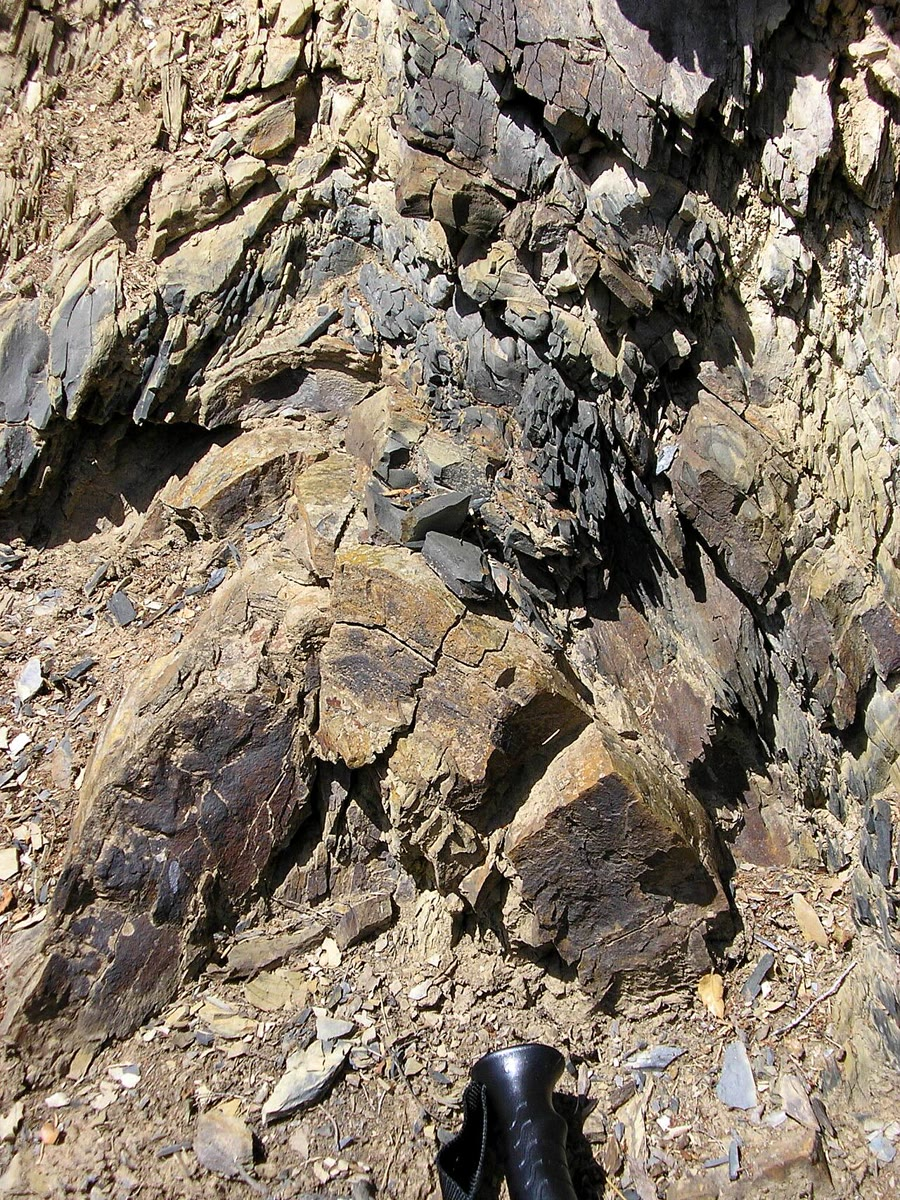
\includegraphics[height=8.2cm]{images/book3/b1-axial-planar-cleavage.jpg}
\par\smallskip{\small Um pequeno \omterm{def:b1:geological-maps:fold}{anticlinal} em arenito e folhelho alternados, de idade carbonífera, perto de Potes, Cantábria. As camadas de arenito marrom se arqueiam sobre a \omterm{def:b1:faults-folds-fabrics:fold-elements}{charneira}, no meio inferior da imagem; no folhelho escuro acima delas, a \omterm{def:b1:faults-folds-fabrics:foliation}{clivagem}, um conjunto de fraturas íngremes e bem espaçadas que atravessam as camadas, é plano-axial: quase paralela ao \omterm{def:b1:faults-folds-fabrics:fold-elements}{plano axial} da \omterm{def:b1:geological-maps:fold}{dobra}, ela se abre através dele, com o leque mudando de camada para camada. O cabo da bengala tem cerca de \qty{4}{cm} de largura.
Foto: Mikenorton, CC~BY-SA~3.0 (Wikimedia Commons).}
\label{fig:b1:faults-folds-fabrics:cleavage}
\end{omfigure}
% ledger: commons:axial-cleavage

\begin{definition}[Lineação, lineação de interseção, lineação de estiramento]\label{def:b1:faults-folds-fabrics:lineation}
Uma \emph{lineação}\index{lineação} é uma fábrica linear que permeia uma rocha, medida por seu \omterm{def:b1:field-lab-methods-1:trend-plunge}{rumo} e \omterm{def:b1:field-lab-methods-1:trend-plunge}{caimento}. Uma \emph{lineação de interseção}\index{lineação de interseção} é o conjunto de linhas ao longo das quais duas fábricas planares se cortam, como o acamamento e uma \omterm{def:b1:faults-folds-fabrics:foliation}{clivagem}; uma \emph{lineação de estiramento}\index{lineação de estiramento} é feita de grãos ou seixos alongados ao longo da \omterm{def:b1:geological-maps:attitude}{direção} de maior \omterm{def:b1:stress-strain-rheology:strain}{alongamento}.
\end{definition}
% ledger: ws:fabrics

\begin{proposition}[Lineação de interseção de uma dobra]\label{prop:b1:faults-folds-fabrics:intersection}
Numa \omterm{def:b1:faults-folds-fabrics:fold-elements}{dobra cilíndrica} com \omterm{def:b1:faults-folds-fabrics:foliation}{clivagem plano-axial}, a \omterm{def:b1:faults-folds-fabrics:lineation}{lineação de interseção} do acamamento e da \omterm{def:b1:faults-folds-fabrics:foliation}{clivagem} é paralela à \omterm{def:b1:faults-folds-fabrics:fold-elements}{linha de charneira}, em toda a \omterm{def:b1:geological-maps:fold}{dobra}.
\end{proposition}

\begin{proof}
Toda superfície de acamamento de uma \omterm{def:b1:faults-folds-fabrics:fold-elements}{dobra cilíndrica} contém a \omterm{def:b1:geological-maps:attitude}{direção} de seu eixo. O \omterm{def:b1:faults-folds-fabrics:fold-elements}{plano axial} contém as \omterm{def:b1:faults-folds-fabrics:fold-elements}{linhas de charneira}, que são paralelas ao eixo, logo contém essa \omterm{def:b1:geological-maps:attitude}{direção} também, e o mesmo ocorre com todo plano de \omterm{def:b1:faults-folds-fabrics:foliation}{clivagem} paralelo a ele. Dois planos que não são paralelos e que contêm a mesma \omterm{def:b1:geological-maps:attitude}{direção} se encontram ao longo de uma linha dessa \omterm{def:b1:geological-maps:attitude}{direção}.
\end{proof}

A proposição é o caminho do geólogo de campo até o \omterm{def:b1:field-lab-methods-1:trend-plunge}{caimento} de uma \omterm{def:b1:geological-maps:fold}{dobra} grande demais para ser vista inteira: em qualquer \omterm{def:b1:geological-maps:geological-map}{afloramento} de um dos \omterm{def:b1:faults-folds-fabrics:fold-elements}{flancos}, as linhas nas quais a \omterm{def:b1:faults-folds-fabrics:foliation}{clivagem} corta o acamamento dão a \omterm{def:b1:faults-folds-fabrics:fold-elements}{linha de charneira}. O acamamento e a \omterm{def:b1:faults-folds-fabrics:foliation}{clivagem} juntos dizem mais: onde está a \omterm{def:b1:geological-maps:fold}{dobra} e de que lado para cima estão as camadas.

\begin{definition}[Vergência]\label{def:b1:faults-folds-fabrics:vergence}
A \emph{vergência}\index{vergência} de uma \omterm{def:b1:geological-maps:fold}{dobra} assimétrica é a \omterm{def:b1:geological-maps:attitude}{direção} horizontal para a qual sua parte superior se moveu em relação à sua parte inferior: a \omterm{def:b1:geological-maps:attitude}{direção} em que ela está invertida ou, para uma \omterm{def:b1:faults-folds-fabrics:fold-classes}{dobra inclinada}, aquela para a qual ela se inclina.
\end{definition}
% ledger: ws:vergence

\begin{proposition}[Acamamento e clivagem nos flancos de uma dobra]\label{prop:b1:faults-folds-fabrics:cleavage-bedding}
Considere uma \omterm{def:b1:geological-maps:fold}{dobra} com \omterm{def:b1:faults-folds-fabrics:fold-elements}{flancos} retos e uma \omterm{def:b1:faults-folds-fabrics:foliation}{clivagem plano-axial}, em rochas que estavam na posição normal antes do dobramento, e em que ambos os \omterm{def:b1:faults-folds-fabrics:fold-elements}{flancos} descem a partir de cada \omterm{def:b1:faults-folds-fabrics:fold-elements}{charneira} \omterm{def:b1:geological-maps:fold}{anticlinal}. Vista no perfil:
\begin{enumerate}[label=(\alph*)]
  \item em um flanco onde o acamamento e a \omterm{def:b1:faults-folds-fabrics:foliation}{clivagem} mergulham para o mesmo lado, o acamamento é o mais íngreme dos dois exatamente quando o flanco está invertido;
  \item a rotação aguda que leva a \omterm{def:b1:faults-folds-fabrics:foliation}{clivagem} sobre o acamamento tem sentidos opostos nos dois \omterm{def:b1:faults-folds-fabrics:fold-elements}{flancos} de uma \omterm{def:b1:geological-maps:fold}{dobra}; em um flanco que não está invertido, ela move o topo da \omterm{def:b1:faults-folds-fabrics:foliation}{clivagem} horizontalmente em direção à \omterm{def:b1:faults-folds-fabrics:fold-elements}{charneira} \omterm{def:b1:geological-maps:fold}{anticlinal} no topo desse flanco.
\end{enumerate}
\end{proposition}

\begin{proof}
Olhe ao longo da \omterm{def:b1:faults-folds-fabrics:fold-elements}{charneira} com o \omterm{def:b1:faults-folds-fabrics:fold-elements}{plano axial} mergulhando para a esquerda com o ângulo $\gamma$, $0 < \gamma \le \ang{90}$, e conte os ângulos no sentido anti-horário a partir da horizontal apontando para a direita. A \omterm{def:b1:faults-folds-fabrics:foliation}{clivagem}, paralela ao \omterm{def:b1:faults-folds-fabrics:fold-elements}{plano axial}, sobe com o ângulo $\gamma$. Em uma \omterm{def:b1:faults-folds-fabrics:fold-elements}{charneira} \omterm{def:b1:geological-maps:fold}{anticlinal}, os dois \omterm{def:b1:faults-folds-fabrics:fold-elements}{flancos} saem para baixo com os ângulos $\ang{180} + \gamma - \iota/2$ (flanco~1) e $\ang{180} + \gamma + \iota/2$ (flanco~2), de cada lado do \omterm{def:b1:faults-folds-fabrics:fold-elements}{plano axial}, com $\iota/2 \le \gamma$ pois ambos descem; todo flanco de uma série de \omterm{def:b1:geological-maps:fold}{dobras} é um desses dois para o \omterm{def:b1:geological-maps:fold}{anticlinal} em seu topo. As rochas ficam mais jovens para fora, afastando-se do núcleo do \omterm{def:b1:geological-maps:fold}{anticlinal}, ao longo da normal ao flanco que aponta para longe do \omterm{def:b1:faults-folds-fabrics:fold-elements}{plano axial}.

O flanco~1 desce para a esquerda: mergulha para a esquerda com $\gamma - \iota/2$, menos íngreme que a \omterm{def:b1:faults-folds-fabrics:foliation}{clivagem}. Sua normal para fora, em $\ang{90} + \gamma -
\iota/2$, aponta para cima: ele está na posição normal. Subindo, faz o ângulo $\gamma - \iota/2$, logo a rotação aguda da \omterm{def:b1:faults-folds-fabrics:foliation}{clivagem} para o acamamento é horária, por $\iota/2$: o topo da \omterm{def:b1:faults-folds-fabrics:foliation}{clivagem} se move para a direita, onde está a \omterm{def:b1:faults-folds-fabrics:fold-elements}{charneira}, pois o flanco sai da \omterm{def:b1:faults-folds-fabrics:fold-elements}{charneira} para a esquerda.

O flanco~2 faz com a horizontal, para cima, o ângulo $\gamma + \iota/2$. Se $\gamma + \iota/2 > \ang{90}$, ele desce para a direita e mergulha para a direita, em sentido oposto à \omterm{def:b1:faults-folds-fabrics:foliation}{clivagem}; sua normal para fora, em $\ang{270} + \gamma +
\iota/2$, tem componente para cima $-\cos(\gamma + \iota/2) > 0$: ele está na posição normal. Se $\gamma + \iota/2 < \ang{90}$, ele desce para a esquerda,
mergulhando para a esquerda com $\gamma + \iota/2$, mais íngreme que a \omterm{def:b1:faults-folds-fabrics:foliation}{clivagem}, e a mesma componente é negativa: o flanco está invertido. Em ambos os casos a rotação aguda da \omterm{def:b1:faults-folds-fabrics:foliation}{clivagem} para o acamamento é anti-horária, por $\iota/2$, e move o topo da \omterm{def:b1:faults-folds-fabrics:foliation}{clivagem} para a esquerda; quando o flanco está na posição normal, ele sai da \omterm{def:b1:faults-folds-fabrics:fold-elements}{charneira} para a direita, de modo que a \omterm{def:b1:faults-folds-fabrics:fold-elements}{charneira} fica à esquerda. Assim, os \omterm{def:b1:faults-folds-fabrics:fold-elements}{flancos} que mergulham para o mesmo lado da \omterm{def:b1:faults-folds-fabrics:foliation}{clivagem} são o flanco~1, menos íngreme, e um flanco~2 invertido, mais íngreme, o que é (a); os sentidos são horários no flanco~1 e anti-horários no flanco~2, o que é (b).
\end{proof}

O sentido da rotação muda, assim, em cada \omterm{def:b1:faults-folds-fabrics:fold-elements}{charneira}, \omterm{def:b1:geological-maps:fold}{anticlinal} ou \omterm{def:b1:geological-maps:fold}{sinclinal}. Um geólogo que o registra ao longo de um percurso encontra as \omterm{def:b1:faults-folds-fabrics:fold-elements}{charneiras} de \omterm{def:b1:geological-maps:fold}{dobras} grandes demais para serem vistas em um só \omterm{def:b1:geological-maps:geological-map}{afloramento} onde o sentido muda, e os \omterm{def:b1:faults-folds-fabrics:fold-elements}{flancos} invertidos onde o acamamento é mais íngreme que a \omterm{def:b1:faults-folds-fabrics:foliation}{clivagem}; a palavra \omterm{def:b1:faults-folds-fabrics:vergence}{vergência} também é usada para esse sentido de rotação, e as inversões da \omterm{def:b1:faults-folds-fabrics:vergence}{vergência} de \omterm{def:b1:geological-maps:fold}{dobras} menores são mapeadas do mesmo modo para encontrar as \omterm{def:b1:faults-folds-fabrics:fold-elements}{charneiras} das \omterm{def:b1:geological-maps:fold}{dobras} maiores: as pequenas \omterm{def:b1:geological-maps:fold}{dobras} nos dois \omterm{def:b1:faults-folds-fabrics:fold-elements}{flancos} de uma grande têm assimetrias opostas, e o traço axial dela passa entre elas.
% ledger: ws:vergence, ws:fold-elements

\begin{omfigure}
\begin{tikzpicture}[>={Stealth[length=5pt]}, font=\small]
% a train of chevron folds seen along the hinge (north into the page, east to the right):
% axial planes dipping 60 deg to the west, interlimb angle 40 deg; long limbs dip 40 deg W
% (the right way up), short limbs 80 deg W (overturned). Short limb: from an anticline hinge H_k,
% length s along 260 deg to the syncline hinge S_k; long limb back up along 40 deg to H_{k+1},
% so that all anticline hinges are level, a wavelength w apart.
% Five bedding surfaces, repeated along the axial direction (similar folds); cleavage parallel to it.
\def\s{2.6}
\pgfmathsetmacro{\sx}{\s*cos(260)}\pgfmathsetmacro{\sy}{\s*sin(260)}
\pgfmathsetmacro{\w}{\sx - \sy/tan(40)}
\pgfmathsetmacro{\hx}{0.62*cos(60)}\pgfmathsetmacro{\hy}{0.62*sin(60)}
\newcommand{\surface}[1]{%
  (-\w+#1*\hx, #1*\hy) \foreach \k in {-1,0,1,2,3} { -- ({\k*\w+\sx+#1*\hx}, {\sy+#1*\hy}) -- ({(\k+1)*\w+#1*\hx}, {#1*\hy}) }}
\begin{scope}
  \clip (0.35,-3.3) rectangle (10.0,2.95);
  \begin{scope}
    \clip \surface{0} -- (12,6) -- (-4,6) -- cycle;
    \clip \surface{4} -- (12,-6) -- (-4,-6) -- cycle;
    \fill[omLithSand!45] (-4,-6) rectangle (12,6);
    \fill[omLithShale!40] \surface{2} -- (12,6) -- (-4,6) -- cycle;
    \fill[omLithSand!45] \surface{3} -- (12,6) -- (-4,6) -- cycle;
    \foreach \c in {-8.0,-7.78,...,13.0} {
      \draw[omDef!85, line width=0.35pt] ({\c-6*cot(60)},-6) -- ({\c+6*cot(60)},6);
    }
  \end{scope}
  \foreach \j in {0,1,2,3,4} { \draw[line width=0.75pt, line join=round] \surface{\j}; }
\end{scope}
% axial traces through the anticline hinges, and labels
\foreach \k in {1,2,3} {
  \draw[omThm, dashed, line width=0.6pt] ({\k*\w-0.5*cos(60)},{-0.5*sin(60)}) -- ({\k*\w+3.6*cos(60)},{3.6*sin(60)});
  \node[omThm, font=\scriptsize, anchor=south] at ({\k*\w+3.6*cos(60)},{3.6*sin(60)}) {anticlinal};
}
\foreach \k in {1,2,3} { \node[omThm, font=\scriptsize, anchor=north] at ({\k*\w+\sx},{\sy-0.15}) {sinclinal}; }
\end{tikzpicture}
\par\smallskip{\small Uma série de \omterm{def:b1:geological-maps:fold}{dobras} em chevron invertidas para a direita, em perfil, com uma \omterm{def:b1:faults-folds-fabrics:foliation}{clivagem plano-axial} (linhas azuis finas), desenhada em escala: planos axiais mergulhando \ang{60} para a esquerda, \omterm{def:b1:faults-folds-fabrics:fold-elements}{ângulo entre flancos} \ang{40}. Os \omterm{def:b1:faults-folds-fabrics:fold-elements}{flancos} longos mergulham \ang{40} para a esquerda, menos íngremes que a \omterm{def:b1:faults-folds-fabrics:foliation}{clivagem}, e estão na posição normal; os \omterm{def:b1:faults-folds-fabrics:fold-elements}{flancos} curtos mergulham \ang{80} para a esquerda, mais íngremes que a \omterm{def:b1:faults-folds-fabrics:foliation}{clivagem}, e estão invertidos. Girar a \omterm{def:b1:faults-folds-fabrics:foliation}{clivagem} sobre o acamamento pelo ângulo agudo é horário em todo flanco longo e anti-horário em todo flanco curto. As \omterm{def:b1:geological-maps:fold}{dobras} vergem para a direita.}
\label{fig:b1:faults-folds-fabrics:vergence}
\end{omfigure}

\section{Microestruturas}\label{sec:b1:faults-folds-fabrics:micro}

Ao microscópio, a deformação de uma rocha aparece em seus grãos. Um grão de quartzo dobrado pelo deslizamento lento de sua rede cristalina não se extingue mais de uma só vez entre \omterm{def:b1:field-lab-methods-1:microscope}{polarizadores cruzados}: à medida que a platina gira, uma faixa escura varre o grão, porque suas partes apontam em direções ligeiramente diferentes. Essa extinção ondulante (\cref{ch:b1:optical-mineralogy}) cresce em intensidade à medida que se aproxima de uma zona de cisalhamento, porque defeitos se acumulam na rede cristalina.
Onde há água, os grãos se dissolvem nas faces onde são mais pressionados, e a matéria dissolvida se deposita onde a tensão é menor, ou é levada embora: essa dissolução por pressão encurta as rochas em baixa temperatura e produz muitas clivagens. Em temperatura mais alta, os grãos deformados são substituídos, enquanto a deformação prossegue, por grãos novos, menores e sem deformação, primeiro ao longo dos antigos contornos de grão: recristalização dinâmica, que reduz o tamanho do grão e produz \omterm{def:b1:faults-folds-fabrics:fault-rocks}{milonitos}. As formas dos grãos deformados e dos \omterm{def:b1:rock-forming-minerals:mineral}{minerais} que crescem em suas sombras também mostram para que lado uma zona de cisalhamento se moveu; esses indicadores de sentido de cisalhamento, e os próprios mecanismos, pertencem ao Livro 5.
% ledger: ws:microstructures, ws:fabrics

\section{Exercícios}

\begin{exercise}[$\star$]\label{exo:b1:faults-folds-fabrics:1}
Dê nome a cada falha pelo \omterm{def:b1:faults-folds-fabrics:fault-elements}{rake} de seu \omterm{def:b1:faults-folds-fabrics:fault-elements}{vetor de deslizamento}, para o plano que mergulha \ang{60}: (a) $r = \ang{-90}$; (b) $r = \ang{85}$; (c) $r = 0$; (d) $r = \ang{180}$; (e) $r = \ang{-40}$. (f) Como se chamaria (b) se seu \omterm{def:b1:geological-maps:attitude}{mergulho} fosse \ang{25}?
% ledger: ar:rake, usgs:fault-types
\end{exercise}

\begin{exercise}[$\star$]\label{exo:b1:faults-folds-fabrics:2}
Uma \omterm{def:b1:faults-folds-fabrics:fault-types}{falha normal} mergulha \ang{55}; seu deslizamento é puramente de \omterm{def:b1:geological-maps:attitude}{mergulho}, com \omterm{def:b1:faults-folds-fabrics:fault-elements}{deslizamento líquido} de \qty{300}{m}. Calcule seu \omterm{def:b1:cross-sections:throw}{rejeito} e seu salto.
\end{exercise}

\begin{exercise}[$\star$]\label{exo:b1:faults-folds-fabrics:3}
Dê o \omterm{def:b1:faults-folds-fabrics:fold-elements}{ângulo entre flancos} e a classe de cada \omterm{def:b1:faults-folds-fabrics:fold-classes}{dobra vertical}, cujos \omterm{def:b1:faults-folds-fabrics:fold-elements}{flancos} mergulham em sentidos opostos: (a) \omterm{def:b1:faults-folds-fabrics:fold-elements}{flancos} mergulhando \ang{35} e \ang{35}; (b) \ang{70} e \ang{75}; (c) \ang{85} e \ang{88}.
% ledger: ws:fold-classes
\end{exercise}

\begin{exercise}[$\star$]\label{exo:b1:faults-folds-fabrics:4}
Um arenito tem \omterm{def:b1:stress-strain-rheology:coulomb}{ângulo de atrito interno} \ang{35}. Segundo a teoria de Anderson, com que ângulos mergulham suas falhas normais e seus empurrões? Que ângulo formam entre si duas \omterm{def:b1:faults-folds-fabrics:fault-types}{falhas transcorrentes} conjugadas?
\end{exercise}

\begin{exercise}[$\star\star$]\label{exo:b1:faults-folds-fabrics:5}
Uma falha tem \omterm{def:b1:geological-maps:attitude}{atitude} $090/50$, e \omterm{def:b1:faults-folds-fabrics:fault-rocks}{estrias} de \omterm{def:b1:faults-folds-fabrics:fault-elements}{rake} \ang{-30} sobre ela; o \omterm{def:b1:faults-folds-fabrics:fault-elements}{deslizamento líquido} é \qty{400}{m}. (a) Calcule as componentes transcorrente e de \omterm{def:b1:geological-maps:attitude}{mergulho}, o \omterm{def:b1:cross-sections:throw}{rejeito} e o salto. (b) Escreva o \omterm{def:b1:faults-folds-fabrics:fault-elements}{vetor de deslizamento} em componentes leste, norte e para cima, e dê seu \omterm{def:b1:field-lab-methods-1:trend-plunge}{rumo} e \omterm{def:b1:field-lab-methods-1:trend-plunge}{caimento}. (c) Dê nome à falha.
\end{exercise}

\begin{exercise}[$\star\star$]\label{exo:b1:faults-folds-fabrics:6}
Duas \omterm{def:b1:faults-folds-fabrics:fault-types}{falhas transcorrentes} verticais de mesma idade têm \omterm{def:b1:geological-maps:attitude}{direção} $020$ e $080$. (a) Segundo Anderson, dê as direções de $\sigma_1$, $\sigma_2$ e $\sigma_3$, e o \omterm{def:b1:stress-strain-rheology:coulomb}{ângulo de atrito interno} da rocha. (b) Qual falha é \omterm{def:b1:faults-folds-fabrics:fault-types}{dextral} e qual é \omterm{def:b1:faults-folds-fabrics:fault-types}{sinistral}? Argumente a partir do encurtamento ao longo de $\sigma_1$.
\end{exercise}

\begin{exercise}[$\star\star$]\label{exo:b1:faults-folds-fabrics:7}
Os dois \omterm{def:b1:faults-folds-fabrics:fold-elements}{flancos} de uma \omterm{def:b1:faults-folds-fabrics:fold-elements}{dobra cilíndrica} têm as \omterm{def:b1:geological-maps:attitude}{atitudes} $120/40$ e $260/30$. Com a \cref{prop:b1:faults-folds-fabrics:hinge}, encontre o \omterm{def:b1:field-lab-methods-1:trend-plunge}{rumo} e o \omterm{def:b1:field-lab-methods-1:trend-plunge}{caimento} de sua \omterm{def:b1:faults-folds-fabrics:fold-elements}{linha de charneira}, seu \omterm{def:b1:faults-folds-fabrics:fold-elements}{ângulo entre flancos} e sua classe.
\end{exercise}

\begin{exercise}[$\star\star$]\label{exo:b1:faults-folds-fabrics:8}
Num \omterm{def:b1:geological-maps:geological-map}{afloramento}, o acamamento tem a \omterm{def:b1:geological-maps:attitude}{atitude} $040/30$ e uma \omterm{def:b1:faults-folds-fabrics:foliation}{clivagem plano-axial} a \omterm{def:b1:geological-maps:attitude}{atitude} $160/80$. Encontre o \omterm{def:b1:field-lab-methods-1:trend-plunge}{rumo} e o \omterm{def:b1:field-lab-methods-1:trend-plunge}{caimento} da \omterm{def:b1:faults-folds-fabrics:lineation}{lineação de interseção}. O que ela diz sobre a \omterm{def:b1:geological-maps:fold}{dobra}?
\end{exercise}

\begin{exercise}[$\star\star$]\label{exo:b1:faults-folds-fabrics:9}
Uma falha vertical tem \omterm{def:b1:geological-maps:attitude}{direção} leste--oeste. Um dique vertical de \omterm{def:b1:geological-maps:attitude}{direção} norte--sul a atravessa; ao norte da falha, o dique é encontrado \qty{350}{m} a leste de onde está ao sul da falha. (a) A falha é \omterm{def:b1:faults-folds-fabrics:fault-types}{dextral} ou \omterm{def:b1:faults-folds-fabrics:fault-types}{sinistral}? (b) Se as \omterm{def:b1:faults-folds-fabrics:fault-rocks}{estrias} forem horizontais, qual é o \omterm{def:b1:faults-folds-fabrics:fault-elements}{deslizamento líquido}? (c) Se, em vez disso, elas caírem \ang{20} para leste, qual são o \omterm{def:b1:faults-folds-fabrics:fault-elements}{deslizamento líquido} e a componente vertical do deslizamento, e qual bloco desceu?
\end{exercise}

\begin{exercise}[$\star\star\star$]\label{exo:b1:faults-folds-fabrics:10}
Uma falha sem \omterm{def:b1:stress-strain-rheology:coulomb}{coesão} e com coeficiente de atrito $\mu$ faz o ângulo $\theta$ com $\sigma_1$. (a) Mostre que ela desliza quando as \omterm{def:b1:stress-strain-rheology:principal}{tensões principais} efetivas atingem a razão
\[
  \frac{\sigma_1'}{\sigma_3'} = \frac{1 + \mu\cot\theta}{1 - \mu\tan\theta} .
\]
(b) Com $\mu = 0.6$ e $\sigma_1$ vertical, calcule a razão para falhas normais que mergulham \ang{60}, \ang{45} e \ang{35}. (c) Mostre que uma \omterm{def:b1:faults-folds-fabrics:fault-types}{falha normal} que mergulha menos que certo ângulo nunca pode deslizar, e calcule esse ângulo. (d) Para $\mu = 0.6$ e $\mu = 0.85$, dê os \omterm{def:b1:geological-maps:attitude}{mergulhos} das falhas normais e de empurrão mais bem orientadas.
\end{exercise}

\begin{exercise}[$\star\star\star$]\label{exo:b1:faults-folds-fabrics:11}
Ao longo de um percurso leste--oeste atravessando \omterm{def:b1:geological-maps:fold}{dobras} em chevron cujas \omterm{def:b1:faults-folds-fabrics:fold-elements}{charneiras} têm \omterm{def:b1:geological-maps:attitude}{direção} norte, um \omterm{def:b1:faults-folds-fabrics:fold-elements}{plano axial} de \omterm{def:b1:faults-folds-fabrics:foliation}{clivagem} mergulha \ang{60} para oeste em toda parte. O acamamento mergulha \ang{40} O na estação A, \ang{80} O na estação B e \ang{40} O na estação C, de oeste para leste, em rochas que estavam na posição normal antes do dobramento. (a) Qual estação está num flanco invertido? (b) Em que sentido a \omterm{def:b1:faults-folds-fabrics:foliation}{clivagem} gira sobre o acamamento em cada estação, vista olhando para o norte? (c) Onde estão as \omterm{def:b1:faults-folds-fabrics:fold-elements}{charneiras}, e quais são anticlinais? (d) Encontre o \omterm{def:b1:faults-folds-fabrics:fold-elements}{ângulo entre flancos} e a \omterm{def:b1:geological-maps:attitude}{atitude} dos planos axiais, e diga para que lado as \omterm{def:b1:geological-maps:fold}{dobras} vergem.
\end{exercise}

\begin{exercise}[$\star\star\star$]\label{exo:b1:faults-folds-fabrics:12}
Uma camada de comprimento $L_0$ é dobrada numa série de \omterm{def:b1:geological-maps:fold}{dobras} em chevron simétricas de \omterm{def:b1:faults-folds-fabrics:fold-elements}{ângulo entre flancos} $\iota$, com seu comprimento inalterado. (a) Mostre que seu comprimento medido através das \omterm{def:b1:geological-maps:fold}{dobras} torna-se $L_0\sin(\iota/2)$. (b) Que encurtamento representam \omterm{def:b1:geological-maps:fold}{dobras} em chevron de \omterm{def:b1:faults-folds-fabrics:fold-elements}{ângulo entre flancos} \ang{60}? (c) Que \omterm{def:b1:faults-folds-fabrics:fold-elements}{ângulo entre flancos} corresponde a um encurtamento de \qty{30}{\percent}? (d) Uma série de \omterm{def:b1:geological-maps:fold}{dobras} verticais com \omterm{def:b1:faults-folds-fabrics:fold-elements}{flancos} mergulhando \ang{12}: qual é o encurtamento?
\end{exercise}

\section{Problema: as estruturas das Colinas de Varden, medidas}

\begin{problem}[{Problema de fim de semana --- o anticlinal e a falha normal das Colinas de Varden, a partir das atitudes de seus planos e do deslizamento sobre a falha}]
\label{pb:b1:faults-folds-fabrics:1}
% values: calc/ch17.py; region: figdata/shared/region.py (limbs, plunge, fault)
As Colinas de Varden estão dobradas em um \omterm{def:b1:geological-maps:fold}{anticlinal}, cujo eixo corre de norte a sul em $x = \qty{3.5}{km}$, e um \omterm{def:b1:geological-maps:fold}{sinclinal} a \qty{4}{km} a leste dele; ambos têm \omterm{def:b1:faults-folds-fabrics:fold-elements}{flancos} planos. Um levantamento de campo mediu o acamamento no flanco leste do \omterm{def:b1:geological-maps:fold}{anticlinal} como $080.7/12.2$ e no flanco oeste como $279.3/12.2$. A cobertura é cortada por uma \omterm{def:b1:faults-folds-fabrics:fault-types}{falha normal} de \omterm{def:b1:geological-maps:attitude}{atitude} $120/60$, cujo \omterm{def:b1:faults-folds-fabrics:fault-elements}{bloco superior} desceu ao longo do \omterm{def:b1:geological-maps:attitude}{mergulho}, com um \omterm{def:b1:cross-sections:throw}{rejeito} de \qty{200}{m}. Dê os ângulos com precisão de \ang{0.1} e os comprimentos com precisão de \qty{0.1}{m}.

\medskip
\noindent\textbf{Parte I --- Os flancos.}
\begin{enumerate}
  \item Escreva as normais unitárias ascendentes $\mathbf n_1$ (flanco leste) e
        $\mathbf n_2$ (flanco oeste) em componentes leste, norte e para cima.
  \item Calcule $\mathbf n_1\cdot\mathbf n_2$ e o ângulo entre as normais.
  \item Deduza o \omterm{def:b1:faults-folds-fabrics:fold-elements}{ângulo entre flancos} do \omterm{def:b1:geological-maps:fold}{anticlinal}.
  \item Classifique o \omterm{def:b1:geological-maps:fold}{anticlinal} pelo seu \omterm{def:b1:faults-folds-fabrics:fold-elements}{ângulo entre flancos}.
  \item Os dois \omterm{def:b1:faults-folds-fabrics:fold-elements}{flancos} mergulham \ang{12.2}. Por que o \omterm{def:b1:faults-folds-fabrics:fold-elements}{ângulo entre flancos} não é exatamente $\ang{180} - 2\times\ang{12.2}$? Calcule o \omterm{def:b1:cross-sections:apparent-dip}{mergulho aparente} de qualquer um dos \omterm{def:b1:faults-folds-fabrics:fold-elements}{flancos} em uma seção vertical leste--oeste.
  \item O \omterm{def:b1:geological-maps:fold}{sinclinal} compartilha o flanco leste do \omterm{def:b1:geological-maps:fold}{anticlinal}, e seu próprio flanco leste é paralelo ao flanco oeste do \omterm{def:b1:geological-maps:fold}{anticlinal}. Qual é o seu \omterm{def:b1:faults-folds-fabrics:fold-elements}{ângulo entre flancos}?
\end{enumerate}

\medskip
\noindent\textbf{Parte II --- A linha de charneira e o plano axial.}
\begin{enumerate}[resume]
  \item Calcule $\mathbf n_1\times\mathbf n_2$, e o \omterm{def:b1:field-lab-methods-1:trend-plunge}{rumo} e o \omterm{def:b1:field-lab-methods-1:trend-plunge}{caimento} da \omterm{def:b1:faults-folds-fabrics:fold-elements}{linha de charneira}.
  \item Dê a \omterm{def:b1:geological-maps:attitude}{atitude} do \omterm{def:b1:faults-folds-fabrics:fold-elements}{plano axial}. O \omterm{def:b1:geological-maps:fold}{anticlinal} é vertical, inclinado ou deitado?
  \item Dê a descrição completa da \omterm{def:b1:geological-maps:fold}{dobra}: aperto, \omterm{def:b1:geological-maps:attitude}{atitude} do \omterm{def:b1:faults-folds-fabrics:fold-elements}{plano axial}, \omterm{def:b1:field-lab-methods-1:trend-plunge}{caimento}.
  \item No \omterm{def:b1:geological-maps:geological-map}{mapa geológico} do \cref{ch:b1:geological-maps}, para que lado fecham os \omterm{def:b1:geological-maps:geological-map}{afloramentos} do \omterm{def:b1:geological-maps:fold}{anticlinal}, e o que aflora em seu núcleo?
  \item O folhelho da cobertura tem uma \omterm{def:b1:faults-folds-fabrics:foliation}{clivagem plano-axial}. Dê sua \omterm{def:b1:geological-maps:attitude}{atitude}, e o \omterm{def:b1:field-lab-methods-1:trend-plunge}{rumo} e o \omterm{def:b1:field-lab-methods-1:trend-plunge}{caimento} de sua \omterm{def:b1:faults-folds-fabrics:lineation}{lineação de interseção} no flanco leste.
  \item No flanco leste, em que sentido a \omterm{def:b1:faults-folds-fabrics:foliation}{clivagem} gira sobre o acamamento, vista olhando para o norte, e de que lado está a \omterm{def:b1:faults-folds-fabrics:fold-elements}{charneira} do \omterm{def:b1:geological-maps:fold}{anticlinal}?
\end{enumerate}

\medskip
\noindent\textbf{Parte III --- A falha e as tensões.}
\begin{enumerate}[resume]
  \item Dê a \omterm{def:b1:geological-maps:attitude}{direção} da falha pela regra da mão direita, e diga de que lado de seu traço jaz o \omterm{def:b1:faults-folds-fabrics:fault-elements}{bloco superior}.
  \item Qual tensão principal era vertical quando a falha se formou, segundo Anderson?
  \item Dê as direções das duas \omterm{def:b1:stress-strain-rheology:principal}{tensões principais} horizontais.
  \item Que \omterm{def:b1:stress-strain-rheology:coulomb}{ângulo de atrito interno} o \omterm{def:b1:geological-maps:attitude}{mergulho} implica? Que \omterm{def:b1:stress-strain-rheology:coulomb}{coeficiente de atrito interno}?
  \item Dê a \omterm{def:b1:geological-maps:attitude}{atitude} do conjunto conjugado de falhas que as mesmas tensões poderiam ter feito, e o ângulo entre os dois conjuntos.
  \item A falha estaria na melhor orientação para deslizar de novo sob o mesmo regime, com o atrito de Byerlee de 0.85?
\end{enumerate}

\medskip
\noindent\textbf{Parte IV --- O deslizamento.}
\begin{enumerate}[resume]
  \item Dê o \omterm{def:b1:faults-folds-fabrics:fault-elements}{rake} do \omterm{def:b1:faults-folds-fabrics:fault-elements}{vetor de deslizamento}, e seu \omterm{def:b1:field-lab-methods-1:trend-plunge}{rumo} e \omterm{def:b1:field-lab-methods-1:trend-plunge}{caimento}.
  \item Escreva o vetor unitário do deslizamento em componentes leste, norte e para cima.
  \item Calcule o salto da falha.
  \item Calcule as componentes leste e norte do deslocamento horizontal do \omterm{def:b1:faults-folds-fabrics:fault-elements}{bloco superior}.
  \item Verifique que o \omterm{def:b1:faults-folds-fabrics:fault-elements}{deslizamento líquido} $L$, o \omterm{def:b1:cross-sections:throw}{rejeito} $h$ e o salto $e$ satisfazem $L^2 = h^2 + e^2$, e explique por quê.
  \item Com aproximação de um metro, qual é o \omterm{def:b1:faults-folds-fabrics:fault-elements}{deslizamento líquido} na falha de Varden?
\end{enumerate}
\end{problem}
